\documentclass[twoside]{book}

% Packages required by doxygen
\usepackage{fixltx2e}
\usepackage{calc}
\usepackage{doxygen}
\usepackage[export]{adjustbox} % also loads graphicx
\usepackage{graphicx}
\usepackage[utf8]{inputenc}
\usepackage{makeidx}
\usepackage{multicol}
\usepackage{multirow}
\PassOptionsToPackage{warn}{textcomp}
\usepackage{textcomp}
\usepackage[nointegrals]{wasysym}
\usepackage[table]{xcolor}

% Font selection
\usepackage[T1]{fontenc}
\usepackage[scaled=.90]{helvet}
\usepackage{courier}
\usepackage{amssymb}
\usepackage{sectsty}
\renewcommand{\familydefault}{\sfdefault}
\allsectionsfont{%
  \fontseries{bc}\selectfont%
  \color{darkgray}%
}
\renewcommand{\DoxyLabelFont}{%
  \fontseries{bc}\selectfont%
  \color{darkgray}%
}
\newcommand{\+}{\discretionary{\mbox{\scriptsize$\hookleftarrow$}}{}{}}

% Page & text layout
\usepackage{geometry}
\geometry{%
  a4paper,%
  top=2.5cm,%
  bottom=2.5cm,%
  left=2.5cm,%
  right=2.5cm%
}
\tolerance=750
\hfuzz=15pt
\hbadness=750
\setlength{\emergencystretch}{15pt}
\setlength{\parindent}{0cm}
\setlength{\parskip}{3ex plus 2ex minus 2ex}
\makeatletter
\renewcommand{\paragraph}{%
  \@startsection{paragraph}{4}{0ex}{-1.0ex}{1.0ex}{%
    \normalfont\normalsize\bfseries\SS@parafont%
  }%
}
\renewcommand{\subparagraph}{%
  \@startsection{subparagraph}{5}{0ex}{-1.0ex}{1.0ex}{%
    \normalfont\normalsize\bfseries\SS@subparafont%
  }%
}
\makeatother

% Headers & footers
\usepackage{fancyhdr}
\pagestyle{fancyplain}
\fancyhead[LE]{\fancyplain{}{\bfseries\thepage}}
\fancyhead[CE]{\fancyplain{}{}}
\fancyhead[RE]{\fancyplain{}{\bfseries\leftmark}}
\fancyhead[LO]{\fancyplain{}{\bfseries\rightmark}}
\fancyhead[CO]{\fancyplain{}{}}
\fancyhead[RO]{\fancyplain{}{\bfseries\thepage}}
\fancyfoot[LE]{\fancyplain{}{}}
\fancyfoot[CE]{\fancyplain{}{}}
\fancyfoot[RE]{\fancyplain{}{\bfseries\scriptsize Generated by Doxygen }}
\fancyfoot[LO]{\fancyplain{}{\bfseries\scriptsize Generated by Doxygen }}
\fancyfoot[CO]{\fancyplain{}{}}
\fancyfoot[RO]{\fancyplain{}{}}
\renewcommand{\footrulewidth}{0.4pt}
\renewcommand{\chaptermark}[1]{%
  \markboth{#1}{}%
}
\renewcommand{\sectionmark}[1]{%
  \markright{\thesection\ #1}%
}

% Indices & bibliography
\usepackage{natbib}
\usepackage[titles]{tocloft}
\setcounter{tocdepth}{3}
\setcounter{secnumdepth}{5}
\makeindex

% Hyperlinks (required, but should be loaded last)
\usepackage{ifpdf}
\ifpdf
  \usepackage[pdftex,pagebackref=true]{hyperref}
\else
  \usepackage[ps2pdf,pagebackref=true]{hyperref}
\fi
\hypersetup{%
  colorlinks=true,%
  linkcolor=blue,%
  citecolor=blue,%
  unicode%
}

% Custom commands
\newcommand{\clearemptydoublepage}{%
  \newpage{\pagestyle{empty}\cleardoublepage}%
}

\usepackage{caption}
\captionsetup{labelsep=space,justification=centering,font={bf},singlelinecheck=off,skip=4pt,position=top}

%===== C O N T E N T S =====

\begin{document}

% Titlepage & ToC
\hypersetup{pageanchor=false,
             bookmarksnumbered=true,
             pdfencoding=unicode
            }
\pagenumbering{alph}
\begin{titlepage}
\vspace*{7cm}
\begin{center}%
{\Large 3D Sculptor }\\
\vspace*{1cm}
{\large Generated by Doxygen 1.8.13}\\
\end{center}
\end{titlepage}
\clearemptydoublepage
\pagenumbering{roman}
\tableofcontents
\clearemptydoublepage
\pagenumbering{arabic}
\hypersetup{pageanchor=true}

%--- Begin generated contents ---
\chapter{Namespace Index}
\section{Namespace List}
Here is a list of all namespaces with brief descriptions\+:\begin{DoxyCompactList}
\item\contentsline{section}{\hyperlink{namespace_ui}{Ui} }{\pageref{namespace_ui}}{}
\end{DoxyCompactList}

\chapter{Hierarchical Index}
\section{Class Hierarchy}
This inheritance list is sorted roughly, but not completely, alphabetically\+:\begin{DoxyCompactList}
\item \contentsline{section}{Figura\+Geometrica}{\pageref{class_figura_geometrica}}{}
\begin{DoxyCompactList}
\item \contentsline{section}{Cut\+Box}{\pageref{class_cut_box}}{}
\item \contentsline{section}{Cut\+Ellipsoid}{\pageref{class_cut_ellipsoid}}{}
\item \contentsline{section}{Cut\+Sphere}{\pageref{class_cut_sphere}}{}
\item \contentsline{section}{Cut\+Voxel}{\pageref{class_cut_voxel}}{}
\item \contentsline{section}{Put\+Box}{\pageref{class_put_box}}{}
\item \contentsline{section}{Put\+Ellipsoid}{\pageref{class_put_ellipsoid}}{}
\item \contentsline{section}{Put\+Sphere}{\pageref{class_put_sphere}}{}
\item \contentsline{section}{Put\+Voxel}{\pageref{class_put_voxel}}{}
\end{DoxyCompactList}
\item Q\+Dialog\begin{DoxyCompactList}
\item \contentsline{section}{box\+Dialog}{\pageref{classbox_dialog}}{}
\item \contentsline{section}{dim\+Dialog}{\pageref{classdim_dialog}}{}
\item \contentsline{section}{Ellipsoid\+Dialog}{\pageref{class_ellipsoid_dialog}}{}
\item \contentsline{section}{Sphere\+Dialog}{\pageref{class_sphere_dialog}}{}
\end{DoxyCompactList}
\item Q\+Main\+Window\begin{DoxyCompactList}
\item \contentsline{section}{Main\+Window}{\pageref{class_main_window}}{}
\end{DoxyCompactList}
\item Q\+Widget\begin{DoxyCompactList}
\item \contentsline{section}{Plotter}{\pageref{class_plotter}}{}
\end{DoxyCompactList}
\item \contentsline{section}{Sculptor}{\pageref{class_sculptor}}{}
\item \contentsline{section}{Voxel}{\pageref{struct_voxel}}{}
\end{DoxyCompactList}

\chapter{Class Index}
\section{Class List}
Here are the classes, structs, unions and interfaces with brief descriptions\+:\begin{DoxyCompactList}
\item\contentsline{section}{\hyperlink{classbox_dialog}{box\+Dialog} }{\pageref{classbox_dialog}}{}
\item\contentsline{section}{\hyperlink{class_cut_box}{Cut\+Box} \\*A classe \hyperlink{class_cut_box}{Cut\+Box} apaga uma caixa no espaço }{\pageref{class_cut_box}}{}
\item\contentsline{section}{\hyperlink{class_cut_ellipsoid}{Cut\+Ellipsoid} \\*A classe \hyperlink{class_cut_ellipsoid}{Cut\+Ellipsoid} apaga um elipsoide no espaço }{\pageref{class_cut_ellipsoid}}{}
\item\contentsline{section}{\hyperlink{class_cut_sphere}{Cut\+Sphere} \\*A classe \hyperlink{class_cut_sphere}{Cut\+Sphere} apaga uma esfera no espaço }{\pageref{class_cut_sphere}}{}
\item\contentsline{section}{\hyperlink{class_cut_voxel}{Cut\+Voxel} \\*A classe \hyperlink{class_cut_voxel}{Cut\+Voxel} apaga um voxel na posição especificada }{\pageref{class_cut_voxel}}{}
\item\contentsline{section}{\hyperlink{classdim_dialog}{dim\+Dialog} }{\pageref{classdim_dialog}}{}
\item\contentsline{section}{\hyperlink{class_ellipsoid_dialog}{Ellipsoid\+Dialog} }{\pageref{class_ellipsoid_dialog}}{}
\item\contentsline{section}{\hyperlink{class_figura_geometrica}{Figura\+Geometrica} \\*A classe \hyperlink{class_figura_geometrica}{Figura\+Geometrica} serce como classe abstrata para criação de outras figuras }{\pageref{class_figura_geometrica}}{}
\item\contentsline{section}{\hyperlink{class_main_window}{Main\+Window} }{\pageref{class_main_window}}{}
\item\contentsline{section}{\hyperlink{class_plotter}{Plotter} }{\pageref{class_plotter}}{}
\item\contentsline{section}{\hyperlink{class_put_box}{Put\+Box} \\*A classe \hyperlink{class_put_box}{Put\+Box} implementa uma caixa no espaço }{\pageref{class_put_box}}{}
\item\contentsline{section}{\hyperlink{class_put_ellipsoid}{Put\+Ellipsoid} \\*A classe \hyperlink{class_put_ellipsoid}{Put\+Ellipsoid} implementa um elipsoide no espaço }{\pageref{class_put_ellipsoid}}{}
\item\contentsline{section}{\hyperlink{class_put_sphere}{Put\+Sphere} \\*A classe \hyperlink{class_put_sphere}{Put\+Sphere} implementa uma esfera no espaço }{\pageref{class_put_sphere}}{}
\item\contentsline{section}{\hyperlink{class_put_voxel}{Put\+Voxel} \\*A classe \hyperlink{class_put_voxel}{Put\+Voxel} implementa um voxel no espaço }{\pageref{class_put_voxel}}{}
\item\contentsline{section}{\hyperlink{class_sculptor}{Sculptor} \\*A classe \hyperlink{class_sculptor}{Sculptor} define o espaço em que os voxels estarão alocados(como se fosse uma \char`\"{}prancheta\char`\"{} de desenho) }{\pageref{class_sculptor}}{}
\item\contentsline{section}{\hyperlink{class_sphere_dialog}{Sphere\+Dialog} }{\pageref{class_sphere_dialog}}{}
\item\contentsline{section}{\hyperlink{struct_voxel}{Voxel} \\*O \hyperlink{struct_voxel}{Voxel} consiste em um cubo localizado no espaço tridimensional que possui cor, transparência e pode ou não estar ativado }{\pageref{struct_voxel}}{}
\end{DoxyCompactList}

\chapter{File Index}
\section{File List}
Here is a list of all files with brief descriptions\+:\begin{DoxyCompactList}
\item\contentsline{section}{\hyperlink{boxdialog_8cpp}{boxdialog.\+cpp} }{\pageref{boxdialog_8cpp}}{}
\item\contentsline{section}{\hyperlink{boxdialog_8h}{boxdialog.\+h} }{\pageref{boxdialog_8h}}{}
\item\contentsline{section}{\hyperlink{cutbox_8cpp}{cutbox.\+cpp} }{\pageref{cutbox_8cpp}}{}
\item\contentsline{section}{\hyperlink{cutbox_8h}{cutbox.\+h} }{\pageref{cutbox_8h}}{}
\item\contentsline{section}{\hyperlink{cutellipsoid_8cpp}{cutellipsoid.\+cpp} }{\pageref{cutellipsoid_8cpp}}{}
\item\contentsline{section}{\hyperlink{cutellipsoid_8h}{cutellipsoid.\+h} }{\pageref{cutellipsoid_8h}}{}
\item\contentsline{section}{\hyperlink{cutsphere_8cpp}{cutsphere.\+cpp} }{\pageref{cutsphere_8cpp}}{}
\item\contentsline{section}{\hyperlink{cutsphere_8h}{cutsphere.\+h} }{\pageref{cutsphere_8h}}{}
\item\contentsline{section}{\hyperlink{cutvoxel_8cpp}{cutvoxel.\+cpp} }{\pageref{cutvoxel_8cpp}}{}
\item\contentsline{section}{\hyperlink{cutvoxel_8h}{cutvoxel.\+h} }{\pageref{cutvoxel_8h}}{}
\item\contentsline{section}{\hyperlink{dimdialog_8cpp}{dimdialog.\+cpp} }{\pageref{dimdialog_8cpp}}{}
\item\contentsline{section}{\hyperlink{dimdialog_8h}{dimdialog.\+h} }{\pageref{dimdialog_8h}}{}
\item\contentsline{section}{\hyperlink{ellipsoiddialog_8cpp}{ellipsoiddialog.\+cpp} }{\pageref{ellipsoiddialog_8cpp}}{}
\item\contentsline{section}{\hyperlink{ellipsoiddialog_8h}{ellipsoiddialog.\+h} }{\pageref{ellipsoiddialog_8h}}{}
\item\contentsline{section}{\hyperlink{figurageometrica_8cpp}{figurageometrica.\+cpp} }{\pageref{figurageometrica_8cpp}}{}
\item\contentsline{section}{\hyperlink{figurageometrica_8h}{figurageometrica.\+h} }{\pageref{figurageometrica_8h}}{}
\item\contentsline{section}{\hyperlink{main_8cpp}{main.\+cpp} }{\pageref{main_8cpp}}{}
\item\contentsline{section}{\hyperlink{mainwindow_8cpp}{mainwindow.\+cpp} }{\pageref{mainwindow_8cpp}}{}
\item\contentsline{section}{\hyperlink{mainwindow_8h}{mainwindow.\+h} }{\pageref{mainwindow_8h}}{}
\item\contentsline{section}{\hyperlink{plotter_8cpp}{plotter.\+cpp} }{\pageref{plotter_8cpp}}{}
\item\contentsline{section}{\hyperlink{plotter_8h}{plotter.\+h} }{\pageref{plotter_8h}}{}
\item\contentsline{section}{\hyperlink{putbox_8cpp}{putbox.\+cpp} }{\pageref{putbox_8cpp}}{}
\item\contentsline{section}{\hyperlink{putbox_8h}{putbox.\+h} }{\pageref{putbox_8h}}{}
\item\contentsline{section}{\hyperlink{putellipsoid_8cpp}{putellipsoid.\+cpp} }{\pageref{putellipsoid_8cpp}}{}
\item\contentsline{section}{\hyperlink{putellipsoid_8h}{putellipsoid.\+h} }{\pageref{putellipsoid_8h}}{}
\item\contentsline{section}{\hyperlink{putsphere_8cpp}{putsphere.\+cpp} }{\pageref{putsphere_8cpp}}{}
\item\contentsline{section}{\hyperlink{putsphere_8h}{putsphere.\+h} }{\pageref{putsphere_8h}}{}
\item\contentsline{section}{\hyperlink{putvoxel_8cpp}{putvoxel.\+cpp} }{\pageref{putvoxel_8cpp}}{}
\item\contentsline{section}{\hyperlink{putvoxel_8h}{putvoxel.\+h} }{\pageref{putvoxel_8h}}{}
\item\contentsline{section}{\hyperlink{_sculptor_8cpp}{Sculptor.\+cpp} }{\pageref{_sculptor_8cpp}}{}
\item\contentsline{section}{\hyperlink{sculptor_8h}{sculptor.\+h} }{\pageref{sculptor_8h}}{}
\item\contentsline{section}{\hyperlink{spheredialog_8cpp}{spheredialog.\+cpp} }{\pageref{spheredialog_8cpp}}{}
\item\contentsline{section}{\hyperlink{spheredialog_8h}{spheredialog.\+h} }{\pageref{spheredialog_8h}}{}
\end{DoxyCompactList}

\chapter{Namespace Documentation}
\hypertarget{namespace_ui}{}\section{Ui Namespace Reference}
\label{namespace_ui}\index{Ui@{Ui}}

\chapter{Class Documentation}
\hypertarget{classbox_dialog}{}\section{box\+Dialog Class Reference}
\label{classbox_dialog}\index{box\+Dialog@{box\+Dialog}}


{\ttfamily \#include $<$boxdialog.\+h$>$}



Inheritance diagram for box\+Dialog\+:
\nopagebreak
\begin{figure}[H]
\begin{center}
\leavevmode
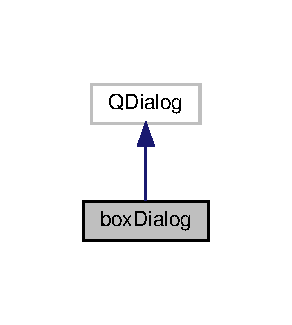
\includegraphics[width=140pt]{classbox_dialog__inherit__graph}
\end{center}
\end{figure}


Collaboration diagram for box\+Dialog\+:
\nopagebreak
\begin{figure}[H]
\begin{center}
\leavevmode
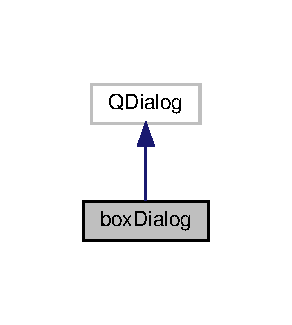
\includegraphics[width=140pt]{classbox_dialog__coll__graph}
\end{center}
\end{figure}
\subsection*{Public Member Functions}
\begin{DoxyCompactItemize}
\item 
\hyperlink{classbox_dialog_ae5f797660638a57b01a9ac34d8c8e6a2}{box\+Dialog} (Q\+Widget $\ast$parent=nullptr)
\item 
\hyperlink{classbox_dialog_aa0f44ec78ac59d41a1d394e9baaa4252}{$\sim$box\+Dialog} ()
\item 
int \hyperlink{classbox_dialog_ab9b74c010cc7b9ab44bf875ae66ede1c}{getX} ()
\item 
int \hyperlink{classbox_dialog_a85e393c20b1187ffdce852378704a24c}{getY} ()
\item 
int \hyperlink{classbox_dialog_a34b2ce0c94a9f2c486d877d64834b7e3}{getZ} ()
\end{DoxyCompactItemize}


\subsection{Constructor \& Destructor Documentation}
\mbox{\Hypertarget{classbox_dialog_ae5f797660638a57b01a9ac34d8c8e6a2}\label{classbox_dialog_ae5f797660638a57b01a9ac34d8c8e6a2}} 
\index{box\+Dialog@{box\+Dialog}!box\+Dialog@{box\+Dialog}}
\index{box\+Dialog@{box\+Dialog}!box\+Dialog@{box\+Dialog}}
\subsubsection{\texorpdfstring{box\+Dialog()}{boxDialog()}}
{\footnotesize\ttfamily box\+Dialog\+::box\+Dialog (\begin{DoxyParamCaption}\item[{Q\+Widget $\ast$}]{parent = {\ttfamily nullptr} }\end{DoxyParamCaption})\hspace{0.3cm}{\ttfamily [explicit]}}

\mbox{\Hypertarget{classbox_dialog_aa0f44ec78ac59d41a1d394e9baaa4252}\label{classbox_dialog_aa0f44ec78ac59d41a1d394e9baaa4252}} 
\index{box\+Dialog@{box\+Dialog}!````~box\+Dialog@{$\sim$box\+Dialog}}
\index{````~box\+Dialog@{$\sim$box\+Dialog}!box\+Dialog@{box\+Dialog}}
\subsubsection{\texorpdfstring{$\sim$box\+Dialog()}{~boxDialog()}}
{\footnotesize\ttfamily box\+Dialog\+::$\sim$box\+Dialog (\begin{DoxyParamCaption}{ }\end{DoxyParamCaption})}



\subsection{Member Function Documentation}
\mbox{\Hypertarget{classbox_dialog_ab9b74c010cc7b9ab44bf875ae66ede1c}\label{classbox_dialog_ab9b74c010cc7b9ab44bf875ae66ede1c}} 
\index{box\+Dialog@{box\+Dialog}!getX@{getX}}
\index{getX@{getX}!box\+Dialog@{box\+Dialog}}
\subsubsection{\texorpdfstring{get\+X()}{getX()}}
{\footnotesize\ttfamily int box\+Dialog\+::getX (\begin{DoxyParamCaption}{ }\end{DoxyParamCaption})}

\mbox{\Hypertarget{classbox_dialog_a85e393c20b1187ffdce852378704a24c}\label{classbox_dialog_a85e393c20b1187ffdce852378704a24c}} 
\index{box\+Dialog@{box\+Dialog}!getY@{getY}}
\index{getY@{getY}!box\+Dialog@{box\+Dialog}}
\subsubsection{\texorpdfstring{get\+Y()}{getY()}}
{\footnotesize\ttfamily int box\+Dialog\+::getY (\begin{DoxyParamCaption}{ }\end{DoxyParamCaption})}

\mbox{\Hypertarget{classbox_dialog_a34b2ce0c94a9f2c486d877d64834b7e3}\label{classbox_dialog_a34b2ce0c94a9f2c486d877d64834b7e3}} 
\index{box\+Dialog@{box\+Dialog}!getZ@{getZ}}
\index{getZ@{getZ}!box\+Dialog@{box\+Dialog}}
\subsubsection{\texorpdfstring{get\+Z()}{getZ()}}
{\footnotesize\ttfamily int box\+Dialog\+::getZ (\begin{DoxyParamCaption}{ }\end{DoxyParamCaption})}



The documentation for this class was generated from the following files\+:\begin{DoxyCompactItemize}
\item 
\hyperlink{boxdialog_8h}{boxdialog.\+h}\item 
\hyperlink{boxdialog_8cpp}{boxdialog.\+cpp}\end{DoxyCompactItemize}

\hypertarget{class_cut_box}{}\section{Cut\+Box Class Reference}
\label{class_cut_box}\index{Cut\+Box@{Cut\+Box}}


A classe \hyperlink{class_cut_box}{Cut\+Box} apaga uma caixa no espaço.  




{\ttfamily \#include $<$cutbox.\+h$>$}



Inheritance diagram for Cut\+Box\+:
\nopagebreak
\begin{figure}[H]
\begin{center}
\leavevmode
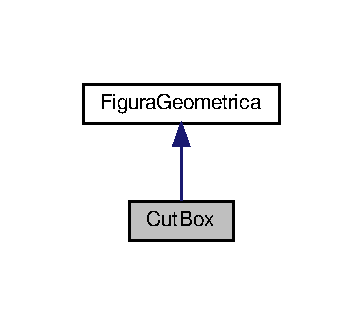
\includegraphics[width=174pt]{class_cut_box__inherit__graph}
\end{center}
\end{figure}


Collaboration diagram for Cut\+Box\+:
\nopagebreak
\begin{figure}[H]
\begin{center}
\leavevmode
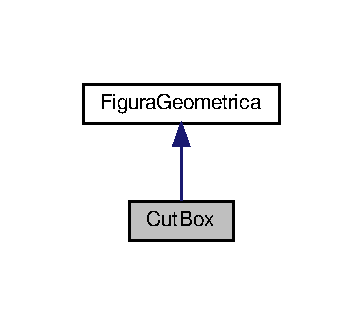
\includegraphics[width=174pt]{class_cut_box__coll__graph}
\end{center}
\end{figure}
\subsection*{Public Member Functions}
\begin{DoxyCompactItemize}
\item 
\hyperlink{class_cut_box_a0e7e856f22e31926719bef5a69685051}{Cut\+Box} (int x0, int x1, int y0, int y1, int z0, int z1)
\begin{DoxyCompactList}\small\item\em \hyperlink{class_cut_box}{Cut\+Box} é o construtor da classe, que recebe como parâmetros os valores iniciais e finais em que deseja apagar a caixa nos eixos(x0,x1,y0,y1,z0,z1) \end{DoxyCompactList}\item 
void \hyperlink{class_cut_box_a01216b04bf5a2d01ce1fb89f3fa62a46}{draw} (\hyperlink{class_sculptor}{Sculptor} \&t)
\begin{DoxyCompactList}\small\item\em draw apaga a caixa para o objeto \hyperlink{class_sculptor}{Sculptor} especificado \end{DoxyCompactList}\end{DoxyCompactItemize}
\subsection*{Additional Inherited Members}


\subsection{Detailed Description}
A classe \hyperlink{class_cut_box}{Cut\+Box} apaga uma caixa no espaço. 

\subsection{Constructor \& Destructor Documentation}
\mbox{\Hypertarget{class_cut_box_a0e7e856f22e31926719bef5a69685051}\label{class_cut_box_a0e7e856f22e31926719bef5a69685051}} 
\index{Cut\+Box@{Cut\+Box}!Cut\+Box@{Cut\+Box}}
\index{Cut\+Box@{Cut\+Box}!Cut\+Box@{Cut\+Box}}
\subsubsection{\texorpdfstring{Cut\+Box()}{CutBox()}}
{\footnotesize\ttfamily Cut\+Box\+::\+Cut\+Box (\begin{DoxyParamCaption}\item[{int}]{x0,  }\item[{int}]{x1,  }\item[{int}]{y0,  }\item[{int}]{y1,  }\item[{int}]{z0,  }\item[{int}]{z1 }\end{DoxyParamCaption})}



\hyperlink{class_cut_box}{Cut\+Box} é o construtor da classe, que recebe como parâmetros os valores iniciais e finais em que deseja apagar a caixa nos eixos(x0,x1,y0,y1,z0,z1) 


\begin{DoxyParams}{Parameters}
{\em x0} & \\
\hline
{\em x1} & \\
\hline
{\em y0} & \\
\hline
{\em y1} & \\
\hline
{\em z0} & \\
\hline
{\em z1} & \\
\hline
\end{DoxyParams}
exemplo de utilização de \hyperlink{class_cut_box}{Cut\+Box}\+: 
\begin{DoxyPre}
\hyperlink{class_cut_box}{CutBox} cb(1,10,1,10,1,10);
\end{DoxyPre}
 

\subsection{Member Function Documentation}
\mbox{\Hypertarget{class_cut_box_a01216b04bf5a2d01ce1fb89f3fa62a46}\label{class_cut_box_a01216b04bf5a2d01ce1fb89f3fa62a46}} 
\index{Cut\+Box@{Cut\+Box}!draw@{draw}}
\index{draw@{draw}!Cut\+Box@{Cut\+Box}}
\subsubsection{\texorpdfstring{draw()}{draw()}}
{\footnotesize\ttfamily void Cut\+Box\+::draw (\begin{DoxyParamCaption}\item[{\hyperlink{class_sculptor}{Sculptor} \&}]{t }\end{DoxyParamCaption})\hspace{0.3cm}{\ttfamily [virtual]}}



draw apaga a caixa para o objeto \hyperlink{class_sculptor}{Sculptor} especificado 


\begin{DoxyParams}{Parameters}
{\em t} & \\
\hline
\end{DoxyParams}


Implements \hyperlink{class_figura_geometrica_a34585fd7c0bd7378fc69c4ee208e676c}{Figura\+Geometrica}.



The documentation for this class was generated from the following files\+:\begin{DoxyCompactItemize}
\item 
\hyperlink{cutbox_8h}{cutbox.\+h}\item 
\hyperlink{cutbox_8cpp}{cutbox.\+cpp}\end{DoxyCompactItemize}

\hypertarget{class_cut_ellipsoid}{}\section{Cut\+Ellipsoid Class Reference}
\label{class_cut_ellipsoid}\index{Cut\+Ellipsoid@{Cut\+Ellipsoid}}


A classe \hyperlink{class_cut_ellipsoid}{Cut\+Ellipsoid} apaga um elipsoide no espaço.  




{\ttfamily \#include $<$cutellipsoid.\+h$>$}



Inheritance diagram for Cut\+Ellipsoid\+:
\nopagebreak
\begin{figure}[H]
\begin{center}
\leavevmode
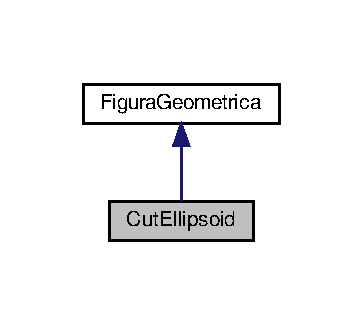
\includegraphics[width=174pt]{class_cut_ellipsoid__inherit__graph}
\end{center}
\end{figure}


Collaboration diagram for Cut\+Ellipsoid\+:
\nopagebreak
\begin{figure}[H]
\begin{center}
\leavevmode
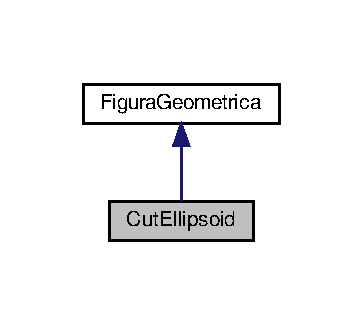
\includegraphics[width=174pt]{class_cut_ellipsoid__coll__graph}
\end{center}
\end{figure}
\subsection*{Public Member Functions}
\begin{DoxyCompactItemize}
\item 
\hyperlink{class_cut_ellipsoid_ad34403f4c6042545d35854f7d2e5db1b}{Cut\+Ellipsoid} (int x, int y, int z, int rx, int ry, int rz)
\begin{DoxyCompactList}\small\item\em \hyperlink{class_cut_ellipsoid}{Cut\+Ellipsoid} é o construtor da classe, que recebe como parâmetros as coordenadas do centro(x,y,z) e os valores dos raios nos eixos(rx,ry,rz) \end{DoxyCompactList}\item 
void \hyperlink{class_cut_ellipsoid_a7110c3cd9dc76bd09ec259b429a3e532}{draw} (\hyperlink{class_sculptor}{Sculptor} \&t)
\begin{DoxyCompactList}\small\item\em draw Apaga a elipsoide para o objeto \hyperlink{class_sculptor}{Sculptor} \end{DoxyCompactList}\end{DoxyCompactItemize}
\subsection*{Additional Inherited Members}


\subsection{Detailed Description}
A classe \hyperlink{class_cut_ellipsoid}{Cut\+Ellipsoid} apaga um elipsoide no espaço. 

\subsection{Constructor \& Destructor Documentation}
\mbox{\Hypertarget{class_cut_ellipsoid_ad34403f4c6042545d35854f7d2e5db1b}\label{class_cut_ellipsoid_ad34403f4c6042545d35854f7d2e5db1b}} 
\index{Cut\+Ellipsoid@{Cut\+Ellipsoid}!Cut\+Ellipsoid@{Cut\+Ellipsoid}}
\index{Cut\+Ellipsoid@{Cut\+Ellipsoid}!Cut\+Ellipsoid@{Cut\+Ellipsoid}}
\subsubsection{\texorpdfstring{Cut\+Ellipsoid()}{CutEllipsoid()}}
{\footnotesize\ttfamily Cut\+Ellipsoid\+::\+Cut\+Ellipsoid (\begin{DoxyParamCaption}\item[{int}]{x,  }\item[{int}]{y,  }\item[{int}]{z,  }\item[{int}]{rx,  }\item[{int}]{ry,  }\item[{int}]{rz }\end{DoxyParamCaption})}



\hyperlink{class_cut_ellipsoid}{Cut\+Ellipsoid} é o construtor da classe, que recebe como parâmetros as coordenadas do centro(x,y,z) e os valores dos raios nos eixos(rx,ry,rz) 


\begin{DoxyParams}{Parameters}
{\em x} & \\
\hline
{\em y} & \\
\hline
{\em z} & \\
\hline
{\em rx} & \\
\hline
{\em ry} & \\
\hline
{\em rz} & \\
\hline
\end{DoxyParams}
Exemplo de utilização da classe \hyperlink{class_cut_ellipsoid}{Cut\+Ellipsoid}\+: 
\begin{DoxyPre}
\hyperlink{class_cut_ellipsoid}{CutEllipsoid} ce(10,10,10,2,3,4)// Apaga Elipsoide centrada em (10,10,10) de raio 2 em,3 em y, 4 em z
\end{DoxyPre}
 

\subsection{Member Function Documentation}
\mbox{\Hypertarget{class_cut_ellipsoid_a7110c3cd9dc76bd09ec259b429a3e532}\label{class_cut_ellipsoid_a7110c3cd9dc76bd09ec259b429a3e532}} 
\index{Cut\+Ellipsoid@{Cut\+Ellipsoid}!draw@{draw}}
\index{draw@{draw}!Cut\+Ellipsoid@{Cut\+Ellipsoid}}
\subsubsection{\texorpdfstring{draw()}{draw()}}
{\footnotesize\ttfamily void Cut\+Ellipsoid\+::draw (\begin{DoxyParamCaption}\item[{\hyperlink{class_sculptor}{Sculptor} \&}]{t }\end{DoxyParamCaption})\hspace{0.3cm}{\ttfamily [virtual]}}



draw Apaga a elipsoide para o objeto \hyperlink{class_sculptor}{Sculptor} 


\begin{DoxyParams}{Parameters}
{\em t} & \\
\hline
\end{DoxyParams}


Implements \hyperlink{class_figura_geometrica_a34585fd7c0bd7378fc69c4ee208e676c}{Figura\+Geometrica}.



The documentation for this class was generated from the following files\+:\begin{DoxyCompactItemize}
\item 
\hyperlink{cutellipsoid_8h}{cutellipsoid.\+h}\item 
\hyperlink{cutellipsoid_8cpp}{cutellipsoid.\+cpp}\end{DoxyCompactItemize}

\hypertarget{class_cut_sphere}{}\section{Cut\+Sphere Class Reference}
\label{class_cut_sphere}\index{Cut\+Sphere@{Cut\+Sphere}}


A classe \hyperlink{class_cut_sphere}{Cut\+Sphere} apaga uma esfera no espaço.  




{\ttfamily \#include $<$cutsphere.\+h$>$}



Inheritance diagram for Cut\+Sphere\+:
\nopagebreak
\begin{figure}[H]
\begin{center}
\leavevmode
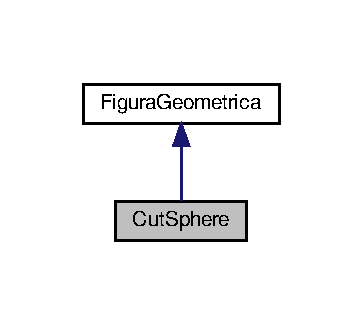
\includegraphics[width=174pt]{class_cut_sphere__inherit__graph}
\end{center}
\end{figure}


Collaboration diagram for Cut\+Sphere\+:
\nopagebreak
\begin{figure}[H]
\begin{center}
\leavevmode
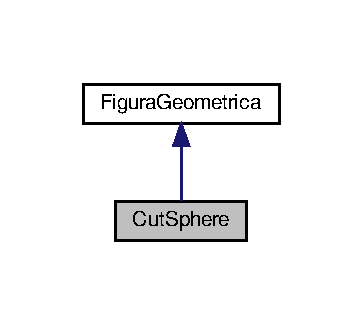
\includegraphics[width=174pt]{class_cut_sphere__coll__graph}
\end{center}
\end{figure}
\subsection*{Public Member Functions}
\begin{DoxyCompactItemize}
\item 
\hyperlink{class_cut_sphere_a7361cbe0f036f9d496e4c83c5b2fea70}{Cut\+Sphere} (int xc, int yc, int zc, int \hyperlink{class_figura_geometrica_a0a4f57efb1a6c525c8aeee34c92e7eab}{r})
\begin{DoxyCompactList}\small\item\em \hyperlink{class_cut_sphere}{Cut\+Sphere} é o construtor da classe, que recebe como parâmetros os valores da coordenada do centro(xc,yc,zc) e o raio. \end{DoxyCompactList}\item 
void \hyperlink{class_cut_sphere_ad62239c047f0817ba6fd4b85ae2eae42}{draw} (\hyperlink{class_sculptor}{Sculptor} \&t)
\begin{DoxyCompactList}\small\item\em draw apaga a esfera para o objeto \hyperlink{class_sculptor}{Sculptor} \end{DoxyCompactList}\end{DoxyCompactItemize}
\subsection*{Additional Inherited Members}


\subsection{Detailed Description}
A classe \hyperlink{class_cut_sphere}{Cut\+Sphere} apaga uma esfera no espaço. 

\subsection{Constructor \& Destructor Documentation}
\mbox{\Hypertarget{class_cut_sphere_a7361cbe0f036f9d496e4c83c5b2fea70}\label{class_cut_sphere_a7361cbe0f036f9d496e4c83c5b2fea70}} 
\index{Cut\+Sphere@{Cut\+Sphere}!Cut\+Sphere@{Cut\+Sphere}}
\index{Cut\+Sphere@{Cut\+Sphere}!Cut\+Sphere@{Cut\+Sphere}}
\subsubsection{\texorpdfstring{Cut\+Sphere()}{CutSphere()}}
{\footnotesize\ttfamily Cut\+Sphere\+::\+Cut\+Sphere (\begin{DoxyParamCaption}\item[{int}]{xc,  }\item[{int}]{yc,  }\item[{int}]{zc,  }\item[{int}]{r }\end{DoxyParamCaption})}



\hyperlink{class_cut_sphere}{Cut\+Sphere} é o construtor da classe, que recebe como parâmetros os valores da coordenada do centro(xc,yc,zc) e o raio. 


\begin{DoxyParams}{Parameters}
{\em xc} & \\
\hline
{\em yc} & \\
\hline
{\em zc} & \\
\hline
{\em r} & \\
\hline
\end{DoxyParams}
Exemplo de utilização de \hyperlink{class_cut_sphere}{Cut\+Sphere}\+: 
\begin{DoxyPre}
\hyperlink{class_cut_sphere}{CutSphere} cs(10,10,10,5);
\end{DoxyPre}
 

\subsection{Member Function Documentation}
\mbox{\Hypertarget{class_cut_sphere_ad62239c047f0817ba6fd4b85ae2eae42}\label{class_cut_sphere_ad62239c047f0817ba6fd4b85ae2eae42}} 
\index{Cut\+Sphere@{Cut\+Sphere}!draw@{draw}}
\index{draw@{draw}!Cut\+Sphere@{Cut\+Sphere}}
\subsubsection{\texorpdfstring{draw()}{draw()}}
{\footnotesize\ttfamily void Cut\+Sphere\+::draw (\begin{DoxyParamCaption}\item[{\hyperlink{class_sculptor}{Sculptor} \&}]{t }\end{DoxyParamCaption})\hspace{0.3cm}{\ttfamily [virtual]}}



draw apaga a esfera para o objeto \hyperlink{class_sculptor}{Sculptor} 


\begin{DoxyParams}{Parameters}
{\em t} & \\
\hline
\end{DoxyParams}


Implements \hyperlink{class_figura_geometrica_a34585fd7c0bd7378fc69c4ee208e676c}{Figura\+Geometrica}.



The documentation for this class was generated from the following files\+:\begin{DoxyCompactItemize}
\item 
\hyperlink{cutsphere_8h}{cutsphere.\+h}\item 
\hyperlink{cutsphere_8cpp}{cutsphere.\+cpp}\end{DoxyCompactItemize}

\hypertarget{class_cut_voxel}{}\section{Cut\+Voxel Class Reference}
\label{class_cut_voxel}\index{Cut\+Voxel@{Cut\+Voxel}}


A classe \hyperlink{class_cut_voxel}{Cut\+Voxel} apaga um voxel na posição especificada.  




{\ttfamily \#include $<$cutvoxel.\+h$>$}



Inheritance diagram for Cut\+Voxel\+:
\nopagebreak
\begin{figure}[H]
\begin{center}
\leavevmode
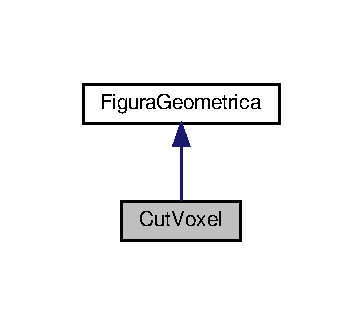
\includegraphics[width=174pt]{class_cut_voxel__inherit__graph}
\end{center}
\end{figure}


Collaboration diagram for Cut\+Voxel\+:
\nopagebreak
\begin{figure}[H]
\begin{center}
\leavevmode
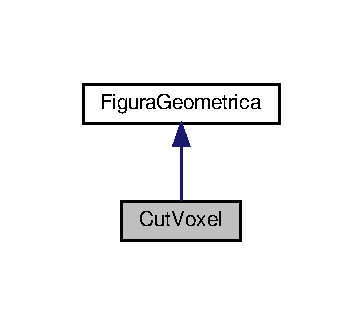
\includegraphics[width=174pt]{class_cut_voxel__coll__graph}
\end{center}
\end{figure}
\subsection*{Public Member Functions}
\begin{DoxyCompactItemize}
\item 
\hyperlink{class_cut_voxel_a32d12f653ebb96da8c3aa62994692bad}{Cut\+Voxel} (int x, int y, int z)
\begin{DoxyCompactList}\small\item\em \hyperlink{class_cut_voxel}{Cut\+Voxel} é o construtor da classe. \end{DoxyCompactList}\item 
void \hyperlink{class_cut_voxel_a4619616e021723dccaf5c7cf12164e01}{draw} (\hyperlink{class_sculptor}{Sculptor} \&t)
\begin{DoxyCompactList}\small\item\em draw apaga o voxel para o objeto \hyperlink{class_sculptor}{Sculptor} \end{DoxyCompactList}\end{DoxyCompactItemize}
\subsection*{Additional Inherited Members}


\subsection{Detailed Description}
A classe \hyperlink{class_cut_voxel}{Cut\+Voxel} apaga um voxel na posição especificada. 

\subsection{Constructor \& Destructor Documentation}
\mbox{\Hypertarget{class_cut_voxel_a32d12f653ebb96da8c3aa62994692bad}\label{class_cut_voxel_a32d12f653ebb96da8c3aa62994692bad}} 
\index{Cut\+Voxel@{Cut\+Voxel}!Cut\+Voxel@{Cut\+Voxel}}
\index{Cut\+Voxel@{Cut\+Voxel}!Cut\+Voxel@{Cut\+Voxel}}
\subsubsection{\texorpdfstring{Cut\+Voxel()}{CutVoxel()}}
{\footnotesize\ttfamily Cut\+Voxel\+::\+Cut\+Voxel (\begin{DoxyParamCaption}\item[{int}]{x,  }\item[{int}]{y,  }\item[{int}]{z }\end{DoxyParamCaption})}



\hyperlink{class_cut_voxel}{Cut\+Voxel} é o construtor da classe. 


\begin{DoxyParams}{Parameters}
{\em x} & \\
\hline
{\em y} & \\
\hline
{\em z} & \\
\hline
\end{DoxyParams}
exemplo de utilização de \hyperlink{class_cut_voxel}{Cut\+Voxel}\+: 
\begin{DoxyPre}
\hyperlink{class_cut_voxel}{CutVoxel} cv(1,1,1); //apaga um voxel na posição (1,1,1)
\end{DoxyPre}
 

\subsection{Member Function Documentation}
\mbox{\Hypertarget{class_cut_voxel_a4619616e021723dccaf5c7cf12164e01}\label{class_cut_voxel_a4619616e021723dccaf5c7cf12164e01}} 
\index{Cut\+Voxel@{Cut\+Voxel}!draw@{draw}}
\index{draw@{draw}!Cut\+Voxel@{Cut\+Voxel}}
\subsubsection{\texorpdfstring{draw()}{draw()}}
{\footnotesize\ttfamily void Cut\+Voxel\+::draw (\begin{DoxyParamCaption}\item[{\hyperlink{class_sculptor}{Sculptor} \&}]{t }\end{DoxyParamCaption})\hspace{0.3cm}{\ttfamily [virtual]}}



draw apaga o voxel para o objeto \hyperlink{class_sculptor}{Sculptor} 


\begin{DoxyParams}{Parameters}
{\em t} & \\
\hline
\end{DoxyParams}


Implements \hyperlink{class_figura_geometrica_a34585fd7c0bd7378fc69c4ee208e676c}{Figura\+Geometrica}.



The documentation for this class was generated from the following files\+:\begin{DoxyCompactItemize}
\item 
\hyperlink{cutvoxel_8h}{cutvoxel.\+h}\item 
\hyperlink{cutvoxel_8cpp}{cutvoxel.\+cpp}\end{DoxyCompactItemize}

\hypertarget{classdim_dialog}{}\section{dim\+Dialog Class Reference}
\label{classdim_dialog}\index{dim\+Dialog@{dim\+Dialog}}


{\ttfamily \#include $<$dimdialog.\+h$>$}



Inheritance diagram for dim\+Dialog\+:
\nopagebreak
\begin{figure}[H]
\begin{center}
\leavevmode
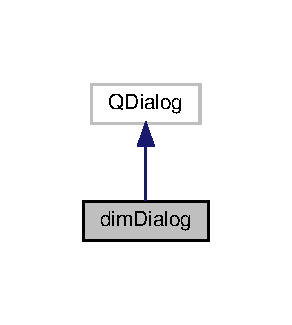
\includegraphics[width=140pt]{classdim_dialog__inherit__graph}
\end{center}
\end{figure}


Collaboration diagram for dim\+Dialog\+:
\nopagebreak
\begin{figure}[H]
\begin{center}
\leavevmode
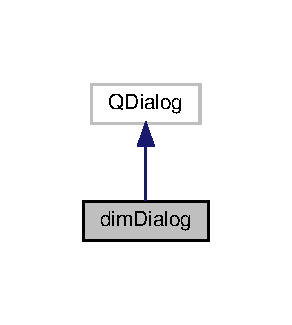
\includegraphics[width=140pt]{classdim_dialog__coll__graph}
\end{center}
\end{figure}
\subsection*{Public Member Functions}
\begin{DoxyCompactItemize}
\item 
\hyperlink{classdim_dialog_abda7437ba444409c789daae87b76202e}{dim\+Dialog} (Q\+Widget $\ast$parent=0)
\item 
\hyperlink{classdim_dialog_a176042f4a3ee628112b5fa1a1737e297}{$\sim$dim\+Dialog} ()
\item 
int \hyperlink{classdim_dialog_a6ad381992f86793368f0b6f2a5c3c32e}{getX} ()
\item 
int \hyperlink{classdim_dialog_abac25538a87509e6486a9427f99cc85b}{getY} ()
\item 
int \hyperlink{classdim_dialog_ac1133f232d42c4e86b68faaa12af98ee}{getZ} ()
\end{DoxyCompactItemize}


\subsection{Constructor \& Destructor Documentation}
\mbox{\Hypertarget{classdim_dialog_abda7437ba444409c789daae87b76202e}\label{classdim_dialog_abda7437ba444409c789daae87b76202e}} 
\index{dim\+Dialog@{dim\+Dialog}!dim\+Dialog@{dim\+Dialog}}
\index{dim\+Dialog@{dim\+Dialog}!dim\+Dialog@{dim\+Dialog}}
\subsubsection{\texorpdfstring{dim\+Dialog()}{dimDialog()}}
{\footnotesize\ttfamily dim\+Dialog\+::dim\+Dialog (\begin{DoxyParamCaption}\item[{Q\+Widget $\ast$}]{parent = {\ttfamily 0} }\end{DoxyParamCaption})\hspace{0.3cm}{\ttfamily [explicit]}}

\mbox{\Hypertarget{classdim_dialog_a176042f4a3ee628112b5fa1a1737e297}\label{classdim_dialog_a176042f4a3ee628112b5fa1a1737e297}} 
\index{dim\+Dialog@{dim\+Dialog}!````~dim\+Dialog@{$\sim$dim\+Dialog}}
\index{````~dim\+Dialog@{$\sim$dim\+Dialog}!dim\+Dialog@{dim\+Dialog}}
\subsubsection{\texorpdfstring{$\sim$dim\+Dialog()}{~dimDialog()}}
{\footnotesize\ttfamily dim\+Dialog\+::$\sim$dim\+Dialog (\begin{DoxyParamCaption}{ }\end{DoxyParamCaption})}



\subsection{Member Function Documentation}
\mbox{\Hypertarget{classdim_dialog_a6ad381992f86793368f0b6f2a5c3c32e}\label{classdim_dialog_a6ad381992f86793368f0b6f2a5c3c32e}} 
\index{dim\+Dialog@{dim\+Dialog}!getX@{getX}}
\index{getX@{getX}!dim\+Dialog@{dim\+Dialog}}
\subsubsection{\texorpdfstring{get\+X()}{getX()}}
{\footnotesize\ttfamily int dim\+Dialog\+::getX (\begin{DoxyParamCaption}{ }\end{DoxyParamCaption})}

\mbox{\Hypertarget{classdim_dialog_abac25538a87509e6486a9427f99cc85b}\label{classdim_dialog_abac25538a87509e6486a9427f99cc85b}} 
\index{dim\+Dialog@{dim\+Dialog}!getY@{getY}}
\index{getY@{getY}!dim\+Dialog@{dim\+Dialog}}
\subsubsection{\texorpdfstring{get\+Y()}{getY()}}
{\footnotesize\ttfamily int dim\+Dialog\+::getY (\begin{DoxyParamCaption}{ }\end{DoxyParamCaption})}

\mbox{\Hypertarget{classdim_dialog_ac1133f232d42c4e86b68faaa12af98ee}\label{classdim_dialog_ac1133f232d42c4e86b68faaa12af98ee}} 
\index{dim\+Dialog@{dim\+Dialog}!getZ@{getZ}}
\index{getZ@{getZ}!dim\+Dialog@{dim\+Dialog}}
\subsubsection{\texorpdfstring{get\+Z()}{getZ()}}
{\footnotesize\ttfamily int dim\+Dialog\+::getZ (\begin{DoxyParamCaption}{ }\end{DoxyParamCaption})}



The documentation for this class was generated from the following files\+:\begin{DoxyCompactItemize}
\item 
\hyperlink{dimdialog_8h}{dimdialog.\+h}\item 
\hyperlink{dimdialog_8cpp}{dimdialog.\+cpp}\end{DoxyCompactItemize}

\hypertarget{class_ellipsoid_dialog}{}\section{Ellipsoid\+Dialog Class Reference}
\label{class_ellipsoid_dialog}\index{Ellipsoid\+Dialog@{Ellipsoid\+Dialog}}


{\ttfamily \#include $<$ellipsoiddialog.\+h$>$}



Inheritance diagram for Ellipsoid\+Dialog\+:
\nopagebreak
\begin{figure}[H]
\begin{center}
\leavevmode
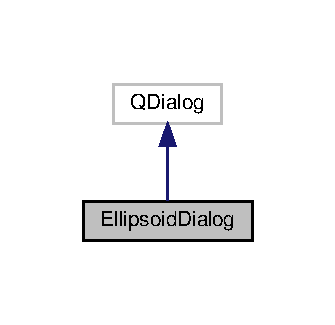
\includegraphics[width=161pt]{class_ellipsoid_dialog__inherit__graph}
\end{center}
\end{figure}


Collaboration diagram for Ellipsoid\+Dialog\+:
\nopagebreak
\begin{figure}[H]
\begin{center}
\leavevmode
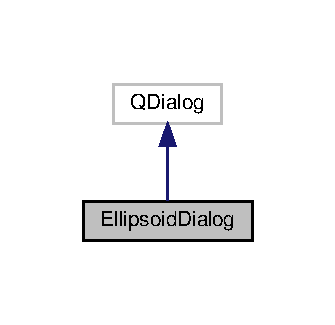
\includegraphics[width=161pt]{class_ellipsoid_dialog__coll__graph}
\end{center}
\end{figure}
\subsection*{Public Member Functions}
\begin{DoxyCompactItemize}
\item 
\hyperlink{class_ellipsoid_dialog_a97f9c450c4c9bf2d4ff189da841516aa}{Ellipsoid\+Dialog} (Q\+Widget $\ast$parent=nullptr)
\item 
int \hyperlink{class_ellipsoid_dialog_aa92ffaab15db5c6efad8716d1d847942}{get\+X\+Radius} ()
\item 
int \hyperlink{class_ellipsoid_dialog_ab9853e51e07c2378aa2464c7be0b9ea2}{get\+Y\+Radius} ()
\item 
int \hyperlink{class_ellipsoid_dialog_ae1cd5fe8262f49b4f158a508fc415ee7}{get\+Z\+Radius} ()
\item 
\hyperlink{class_ellipsoid_dialog_a255484045ff62f4380e5fcdf11ecc2e4}{$\sim$\+Ellipsoid\+Dialog} ()
\end{DoxyCompactItemize}


\subsection{Constructor \& Destructor Documentation}
\mbox{\Hypertarget{class_ellipsoid_dialog_a97f9c450c4c9bf2d4ff189da841516aa}\label{class_ellipsoid_dialog_a97f9c450c4c9bf2d4ff189da841516aa}} 
\index{Ellipsoid\+Dialog@{Ellipsoid\+Dialog}!Ellipsoid\+Dialog@{Ellipsoid\+Dialog}}
\index{Ellipsoid\+Dialog@{Ellipsoid\+Dialog}!Ellipsoid\+Dialog@{Ellipsoid\+Dialog}}
\subsubsection{\texorpdfstring{Ellipsoid\+Dialog()}{EllipsoidDialog()}}
{\footnotesize\ttfamily Ellipsoid\+Dialog\+::\+Ellipsoid\+Dialog (\begin{DoxyParamCaption}\item[{Q\+Widget $\ast$}]{parent = {\ttfamily nullptr} }\end{DoxyParamCaption})\hspace{0.3cm}{\ttfamily [explicit]}}

\mbox{\Hypertarget{class_ellipsoid_dialog_a255484045ff62f4380e5fcdf11ecc2e4}\label{class_ellipsoid_dialog_a255484045ff62f4380e5fcdf11ecc2e4}} 
\index{Ellipsoid\+Dialog@{Ellipsoid\+Dialog}!````~Ellipsoid\+Dialog@{$\sim$\+Ellipsoid\+Dialog}}
\index{````~Ellipsoid\+Dialog@{$\sim$\+Ellipsoid\+Dialog}!Ellipsoid\+Dialog@{Ellipsoid\+Dialog}}
\subsubsection{\texorpdfstring{$\sim$\+Ellipsoid\+Dialog()}{~EllipsoidDialog()}}
{\footnotesize\ttfamily Ellipsoid\+Dialog\+::$\sim$\+Ellipsoid\+Dialog (\begin{DoxyParamCaption}{ }\end{DoxyParamCaption})}



\subsection{Member Function Documentation}
\mbox{\Hypertarget{class_ellipsoid_dialog_aa92ffaab15db5c6efad8716d1d847942}\label{class_ellipsoid_dialog_aa92ffaab15db5c6efad8716d1d847942}} 
\index{Ellipsoid\+Dialog@{Ellipsoid\+Dialog}!get\+X\+Radius@{get\+X\+Radius}}
\index{get\+X\+Radius@{get\+X\+Radius}!Ellipsoid\+Dialog@{Ellipsoid\+Dialog}}
\subsubsection{\texorpdfstring{get\+X\+Radius()}{getXRadius()}}
{\footnotesize\ttfamily int Ellipsoid\+Dialog\+::get\+X\+Radius (\begin{DoxyParamCaption}{ }\end{DoxyParamCaption})}

\mbox{\Hypertarget{class_ellipsoid_dialog_ab9853e51e07c2378aa2464c7be0b9ea2}\label{class_ellipsoid_dialog_ab9853e51e07c2378aa2464c7be0b9ea2}} 
\index{Ellipsoid\+Dialog@{Ellipsoid\+Dialog}!get\+Y\+Radius@{get\+Y\+Radius}}
\index{get\+Y\+Radius@{get\+Y\+Radius}!Ellipsoid\+Dialog@{Ellipsoid\+Dialog}}
\subsubsection{\texorpdfstring{get\+Y\+Radius()}{getYRadius()}}
{\footnotesize\ttfamily int Ellipsoid\+Dialog\+::get\+Y\+Radius (\begin{DoxyParamCaption}{ }\end{DoxyParamCaption})}

\mbox{\Hypertarget{class_ellipsoid_dialog_ae1cd5fe8262f49b4f158a508fc415ee7}\label{class_ellipsoid_dialog_ae1cd5fe8262f49b4f158a508fc415ee7}} 
\index{Ellipsoid\+Dialog@{Ellipsoid\+Dialog}!get\+Z\+Radius@{get\+Z\+Radius}}
\index{get\+Z\+Radius@{get\+Z\+Radius}!Ellipsoid\+Dialog@{Ellipsoid\+Dialog}}
\subsubsection{\texorpdfstring{get\+Z\+Radius()}{getZRadius()}}
{\footnotesize\ttfamily int Ellipsoid\+Dialog\+::get\+Z\+Radius (\begin{DoxyParamCaption}{ }\end{DoxyParamCaption})}



The documentation for this class was generated from the following files\+:\begin{DoxyCompactItemize}
\item 
\hyperlink{ellipsoiddialog_8h}{ellipsoiddialog.\+h}\item 
\hyperlink{ellipsoiddialog_8cpp}{ellipsoiddialog.\+cpp}\end{DoxyCompactItemize}

\hypertarget{class_figura_geometrica}{}\section{Figura\+Geometrica Class Reference}
\label{class_figura_geometrica}\index{Figura\+Geometrica@{Figura\+Geometrica}}


A classe \hyperlink{class_figura_geometrica}{Figura\+Geometrica} serce como classe abstrata para criação de outras figuras.  




{\ttfamily \#include $<$figurageometrica.\+h$>$}



Inheritance diagram for Figura\+Geometrica\+:
\nopagebreak
\begin{figure}[H]
\begin{center}
\leavevmode
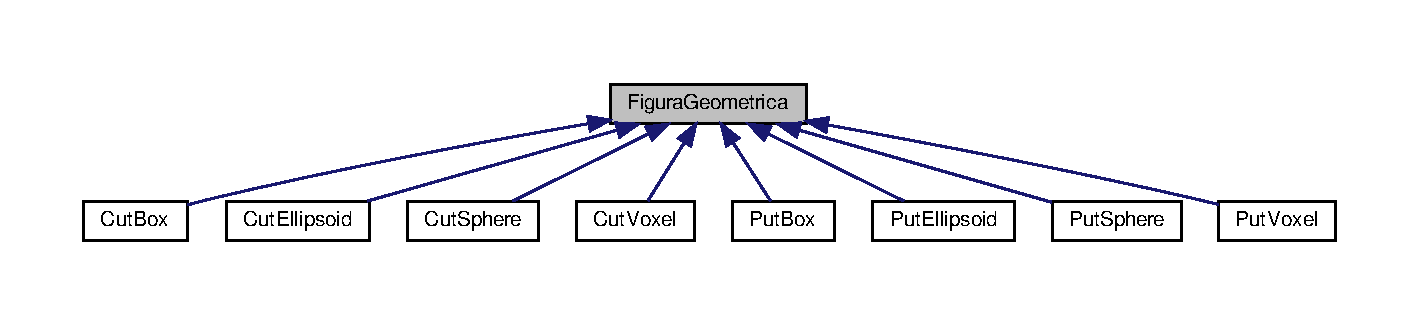
\includegraphics[width=350pt]{class_figura_geometrica__inherit__graph}
\end{center}
\end{figure}
\subsection*{Public Member Functions}
\begin{DoxyCompactItemize}
\item 
\hyperlink{class_figura_geometrica_a81d7c7efaea511e60a15f5a363138dd9}{Figura\+Geometrica} ()
\begin{DoxyCompactList}\small\item\em \hyperlink{class_figura_geometrica}{Figura\+Geometrica} é o contrutor da classe. \end{DoxyCompactList}\item 
virtual void \hyperlink{class_figura_geometrica_a34585fd7c0bd7378fc69c4ee208e676c}{draw} (\hyperlink{class_sculptor}{Sculptor} \&t)=0
\begin{DoxyCompactList}\small\item\em draw é um método que desenha a figura para o objeto \hyperlink{class_sculptor}{Sculptor} especificado \end{DoxyCompactList}\item 
virtual \hyperlink{class_figura_geometrica_ad13b9bccf1b14f6b9fbc662aad61ffd1}{$\sim$\+Figura\+Geometrica} ()
\begin{DoxyCompactList}\small\item\em $\sim$\+Figura\+Geometrica é o destrutor da classe \end{DoxyCompactList}\end{DoxyCompactItemize}
\subsection*{Protected Attributes}
\begin{DoxyCompactItemize}
\item 
float \hyperlink{class_figura_geometrica_a0a4f57efb1a6c525c8aeee34c92e7eab}{r}
\begin{DoxyCompactList}\small\item\em r\+: intensidade da cor vermelha \end{DoxyCompactList}\item 
float \hyperlink{class_figura_geometrica_a51930549bcb90d016b824f10f95df355}{g}
\begin{DoxyCompactList}\small\item\em g\+: intensidade da cor verde \end{DoxyCompactList}\item 
float \hyperlink{class_figura_geometrica_a25e5d6c21410103c25ec55c0117dac0d}{b}
\begin{DoxyCompactList}\small\item\em b\+: intensidade da cor azul \end{DoxyCompactList}\item 
float \hyperlink{class_figura_geometrica_ae7c8a027fcec3c357265b90458a4d165}{a}
\begin{DoxyCompactList}\small\item\em a\+: opacidade(alpha) \end{DoxyCompactList}\end{DoxyCompactItemize}


\subsection{Detailed Description}
A classe \hyperlink{class_figura_geometrica}{Figura\+Geometrica} serce como classe abstrata para criação de outras figuras. 

\hyperlink{class_figura_geometrica}{Figura\+Geometrica} permite que endereços de objetos de classes derivadas dela sejam armazenados em ponteiros dessa classe 

\subsection{Constructor \& Destructor Documentation}
\mbox{\Hypertarget{class_figura_geometrica_a81d7c7efaea511e60a15f5a363138dd9}\label{class_figura_geometrica_a81d7c7efaea511e60a15f5a363138dd9}} 
\index{Figura\+Geometrica@{Figura\+Geometrica}!Figura\+Geometrica@{Figura\+Geometrica}}
\index{Figura\+Geometrica@{Figura\+Geometrica}!Figura\+Geometrica@{Figura\+Geometrica}}
\subsubsection{\texorpdfstring{Figura\+Geometrica()}{FiguraGeometrica()}}
{\footnotesize\ttfamily Figura\+Geometrica\+::\+Figura\+Geometrica (\begin{DoxyParamCaption}{ }\end{DoxyParamCaption})}



\hyperlink{class_figura_geometrica}{Figura\+Geometrica} é o contrutor da classe. 

\mbox{\Hypertarget{class_figura_geometrica_ad13b9bccf1b14f6b9fbc662aad61ffd1}\label{class_figura_geometrica_ad13b9bccf1b14f6b9fbc662aad61ffd1}} 
\index{Figura\+Geometrica@{Figura\+Geometrica}!````~Figura\+Geometrica@{$\sim$\+Figura\+Geometrica}}
\index{````~Figura\+Geometrica@{$\sim$\+Figura\+Geometrica}!Figura\+Geometrica@{Figura\+Geometrica}}
\subsubsection{\texorpdfstring{$\sim$\+Figura\+Geometrica()}{~FiguraGeometrica()}}
{\footnotesize\ttfamily Figura\+Geometrica\+::$\sim$\+Figura\+Geometrica (\begin{DoxyParamCaption}{ }\end{DoxyParamCaption})\hspace{0.3cm}{\ttfamily [virtual]}}



$\sim$\+Figura\+Geometrica é o destrutor da classe 



\subsection{Member Function Documentation}
\mbox{\Hypertarget{class_figura_geometrica_a34585fd7c0bd7378fc69c4ee208e676c}\label{class_figura_geometrica_a34585fd7c0bd7378fc69c4ee208e676c}} 
\index{Figura\+Geometrica@{Figura\+Geometrica}!draw@{draw}}
\index{draw@{draw}!Figura\+Geometrica@{Figura\+Geometrica}}
\subsubsection{\texorpdfstring{draw()}{draw()}}
{\footnotesize\ttfamily virtual void Figura\+Geometrica\+::draw (\begin{DoxyParamCaption}\item[{\hyperlink{class_sculptor}{Sculptor} \&}]{t }\end{DoxyParamCaption})\hspace{0.3cm}{\ttfamily [pure virtual]}}



draw é um método que desenha a figura para o objeto \hyperlink{class_sculptor}{Sculptor} especificado 


\begin{DoxyParams}{Parameters}
{\em t} & \\
\hline
\end{DoxyParams}


Implemented in \hyperlink{class_put_sphere_a5105d1e171563e16c148d8f715321b24}{Put\+Sphere}, \hyperlink{class_put_voxel_af784ab77d8a7aac2010e608796710ccb}{Put\+Voxel}, \hyperlink{class_put_ellipsoid_a961faff306dad93a4b68a35ad9c3027b}{Put\+Ellipsoid}, \hyperlink{class_put_box_a3caaf01d035f5a0749fd308e9a86de94}{Put\+Box}, \hyperlink{class_cut_ellipsoid_a7110c3cd9dc76bd09ec259b429a3e532}{Cut\+Ellipsoid}, \hyperlink{class_cut_box_a01216b04bf5a2d01ce1fb89f3fa62a46}{Cut\+Box}, \hyperlink{class_cut_sphere_ad62239c047f0817ba6fd4b85ae2eae42}{Cut\+Sphere}, and \hyperlink{class_cut_voxel_a4619616e021723dccaf5c7cf12164e01}{Cut\+Voxel}.



\subsection{Member Data Documentation}
\mbox{\Hypertarget{class_figura_geometrica_ae7c8a027fcec3c357265b90458a4d165}\label{class_figura_geometrica_ae7c8a027fcec3c357265b90458a4d165}} 
\index{Figura\+Geometrica@{Figura\+Geometrica}!a@{a}}
\index{a@{a}!Figura\+Geometrica@{Figura\+Geometrica}}
\subsubsection{\texorpdfstring{a}{a}}
{\footnotesize\ttfamily float Figura\+Geometrica\+::a\hspace{0.3cm}{\ttfamily [protected]}}



a\+: opacidade(alpha) 

\mbox{\Hypertarget{class_figura_geometrica_a25e5d6c21410103c25ec55c0117dac0d}\label{class_figura_geometrica_a25e5d6c21410103c25ec55c0117dac0d}} 
\index{Figura\+Geometrica@{Figura\+Geometrica}!b@{b}}
\index{b@{b}!Figura\+Geometrica@{Figura\+Geometrica}}
\subsubsection{\texorpdfstring{b}{b}}
{\footnotesize\ttfamily float Figura\+Geometrica\+::b\hspace{0.3cm}{\ttfamily [protected]}}



b\+: intensidade da cor azul 

\mbox{\Hypertarget{class_figura_geometrica_a51930549bcb90d016b824f10f95df355}\label{class_figura_geometrica_a51930549bcb90d016b824f10f95df355}} 
\index{Figura\+Geometrica@{Figura\+Geometrica}!g@{g}}
\index{g@{g}!Figura\+Geometrica@{Figura\+Geometrica}}
\subsubsection{\texorpdfstring{g}{g}}
{\footnotesize\ttfamily float Figura\+Geometrica\+::g\hspace{0.3cm}{\ttfamily [protected]}}



g\+: intensidade da cor verde 

\mbox{\Hypertarget{class_figura_geometrica_a0a4f57efb1a6c525c8aeee34c92e7eab}\label{class_figura_geometrica_a0a4f57efb1a6c525c8aeee34c92e7eab}} 
\index{Figura\+Geometrica@{Figura\+Geometrica}!r@{r}}
\index{r@{r}!Figura\+Geometrica@{Figura\+Geometrica}}
\subsubsection{\texorpdfstring{r}{r}}
{\footnotesize\ttfamily float Figura\+Geometrica\+::r\hspace{0.3cm}{\ttfamily [protected]}}



r\+: intensidade da cor vermelha 



The documentation for this class was generated from the following files\+:\begin{DoxyCompactItemize}
\item 
\hyperlink{figurageometrica_8h}{figurageometrica.\+h}\item 
\hyperlink{figurageometrica_8cpp}{figurageometrica.\+cpp}\end{DoxyCompactItemize}

\hypertarget{class_main_window}{}\section{Main\+Window Class Reference}
\label{class_main_window}\index{Main\+Window@{Main\+Window}}


{\ttfamily \#include $<$mainwindow.\+h$>$}



Inheritance diagram for Main\+Window\+:
\nopagebreak
\begin{figure}[H]
\begin{center}
\leavevmode
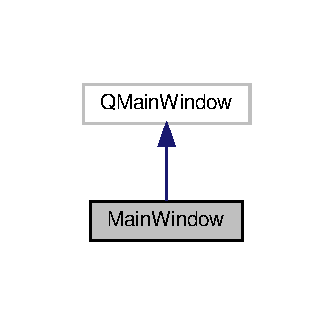
\includegraphics[width=160pt]{class_main_window__inherit__graph}
\end{center}
\end{figure}


Collaboration diagram for Main\+Window\+:
\nopagebreak
\begin{figure}[H]
\begin{center}
\leavevmode
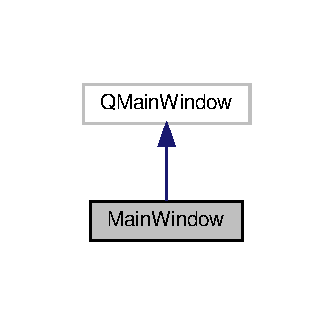
\includegraphics[width=160pt]{class_main_window__coll__graph}
\end{center}
\end{figure}
\subsection*{Public Slots}
\begin{DoxyCompactItemize}
\item 
void \hyperlink{class_main_window_adc0db0162938df94fcb275684e6575a7}{on\+\_\+push\+Button\+Dim\+\_\+clicked} ()
\item 
void \hyperlink{class_main_window_affe842d33f32e0433f150f1a5acef774}{on\+\_\+push\+Button\+Cut\+Box\+\_\+clicked} ()
\end{DoxyCompactItemize}
\subsection*{Public Member Functions}
\begin{DoxyCompactItemize}
\item 
\hyperlink{class_main_window_a8b244be8b7b7db1b08de2a2acb9409db}{Main\+Window} (Q\+Widget $\ast$parent=0)
\item 
\hyperlink{class_main_window_ae98d00a93bc118200eeef9f9bba1dba7}{$\sim$\+Main\+Window} ()
\item 
void \hyperlink{class_main_window_ad82150906607387d5801606dba6495ac}{muda\+Cor} ()
\end{DoxyCompactItemize}


\subsection{Constructor \& Destructor Documentation}
\mbox{\Hypertarget{class_main_window_a8b244be8b7b7db1b08de2a2acb9409db}\label{class_main_window_a8b244be8b7b7db1b08de2a2acb9409db}} 
\index{Main\+Window@{Main\+Window}!Main\+Window@{Main\+Window}}
\index{Main\+Window@{Main\+Window}!Main\+Window@{Main\+Window}}
\subsubsection{\texorpdfstring{Main\+Window()}{MainWindow()}}
{\footnotesize\ttfamily Main\+Window\+::\+Main\+Window (\begin{DoxyParamCaption}\item[{Q\+Widget $\ast$}]{parent = {\ttfamily 0} }\end{DoxyParamCaption})\hspace{0.3cm}{\ttfamily [explicit]}}

\mbox{\Hypertarget{class_main_window_ae98d00a93bc118200eeef9f9bba1dba7}\label{class_main_window_ae98d00a93bc118200eeef9f9bba1dba7}} 
\index{Main\+Window@{Main\+Window}!````~Main\+Window@{$\sim$\+Main\+Window}}
\index{````~Main\+Window@{$\sim$\+Main\+Window}!Main\+Window@{Main\+Window}}
\subsubsection{\texorpdfstring{$\sim$\+Main\+Window()}{~MainWindow()}}
{\footnotesize\ttfamily Main\+Window\+::$\sim$\+Main\+Window (\begin{DoxyParamCaption}{ }\end{DoxyParamCaption})}



\subsection{Member Function Documentation}
\mbox{\Hypertarget{class_main_window_ad82150906607387d5801606dba6495ac}\label{class_main_window_ad82150906607387d5801606dba6495ac}} 
\index{Main\+Window@{Main\+Window}!muda\+Cor@{muda\+Cor}}
\index{muda\+Cor@{muda\+Cor}!Main\+Window@{Main\+Window}}
\subsubsection{\texorpdfstring{muda\+Cor()}{mudaCor()}}
{\footnotesize\ttfamily void Main\+Window\+::muda\+Cor (\begin{DoxyParamCaption}{ }\end{DoxyParamCaption})}

\mbox{\Hypertarget{class_main_window_affe842d33f32e0433f150f1a5acef774}\label{class_main_window_affe842d33f32e0433f150f1a5acef774}} 
\index{Main\+Window@{Main\+Window}!on\+\_\+push\+Button\+Cut\+Box\+\_\+clicked@{on\+\_\+push\+Button\+Cut\+Box\+\_\+clicked}}
\index{on\+\_\+push\+Button\+Cut\+Box\+\_\+clicked@{on\+\_\+push\+Button\+Cut\+Box\+\_\+clicked}!Main\+Window@{Main\+Window}}
\subsubsection{\texorpdfstring{on\+\_\+push\+Button\+Cut\+Box\+\_\+clicked}{on\_pushButtonCutBox\_clicked}}
{\footnotesize\ttfamily void Main\+Window\+::on\+\_\+push\+Button\+Cut\+Box\+\_\+clicked (\begin{DoxyParamCaption}{ }\end{DoxyParamCaption})\hspace{0.3cm}{\ttfamily [slot]}}

\mbox{\Hypertarget{class_main_window_adc0db0162938df94fcb275684e6575a7}\label{class_main_window_adc0db0162938df94fcb275684e6575a7}} 
\index{Main\+Window@{Main\+Window}!on\+\_\+push\+Button\+Dim\+\_\+clicked@{on\+\_\+push\+Button\+Dim\+\_\+clicked}}
\index{on\+\_\+push\+Button\+Dim\+\_\+clicked@{on\+\_\+push\+Button\+Dim\+\_\+clicked}!Main\+Window@{Main\+Window}}
\subsubsection{\texorpdfstring{on\+\_\+push\+Button\+Dim\+\_\+clicked}{on\_pushButtonDim\_clicked}}
{\footnotesize\ttfamily void Main\+Window\+::on\+\_\+push\+Button\+Dim\+\_\+clicked (\begin{DoxyParamCaption}{ }\end{DoxyParamCaption})\hspace{0.3cm}{\ttfamily [slot]}}



The documentation for this class was generated from the following files\+:\begin{DoxyCompactItemize}
\item 
\hyperlink{mainwindow_8h}{mainwindow.\+h}\item 
\hyperlink{mainwindow_8cpp}{mainwindow.\+cpp}\end{DoxyCompactItemize}

\hypertarget{class_plotter}{}\section{Plotter Class Reference}
\label{class_plotter}\index{Plotter@{Plotter}}


{\ttfamily \#include $<$plotter.\+h$>$}



Inheritance diagram for Plotter\+:
\nopagebreak
\begin{figure}[H]
\begin{center}
\leavevmode
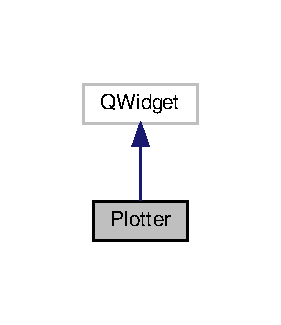
\includegraphics[width=135pt]{class_plotter__inherit__graph}
\end{center}
\end{figure}


Collaboration diagram for Plotter\+:
\nopagebreak
\begin{figure}[H]
\begin{center}
\leavevmode
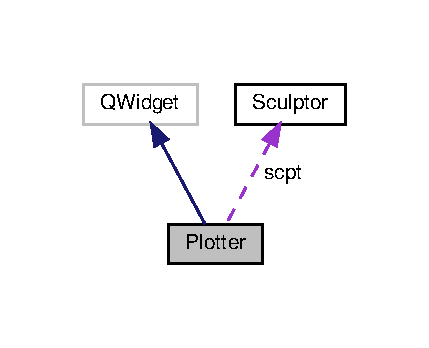
\includegraphics[width=206pt]{class_plotter__coll__graph}
\end{center}
\end{figure}
\subsection*{Public Slots}
\begin{DoxyCompactItemize}
\item 
void \hyperlink{class_plotter_a6f80702bdfaef06fc3c127bcf2e92b45}{setdrawmodule} (int)
\item 
void \hyperlink{class_plotter_aa2706e1b6da1cdde9c5dcfcf001215c1}{setplan} (int)
\end{DoxyCompactItemize}
\subsection*{Signals}
\begin{DoxyCompactItemize}
\item 
void \hyperlink{class_plotter_acc318f23eb9f135d13431c05221e1ee9}{mouseX} (int)
\item 
void \hyperlink{class_plotter_ae66c4db3fec253319af537aa627d8f1b}{mouseY} (int)
\end{DoxyCompactItemize}
\subsection*{Public Member Functions}
\begin{DoxyCompactItemize}
\item 
\hyperlink{class_plotter_a1807627530de30ae58dff3c42a823497}{Plotter} (Q\+Widget $\ast$parent=nullptr)
\item 
void \hyperlink{class_plotter_a06477bf987646f000a8982db1352a11d}{paint\+Event} (Q\+Paint\+Event $\ast$event)
\item 
void \hyperlink{class_plotter_aac8dfc9c49d06ccf085973ceec6eb50c}{mouse\+Press\+Event} (Q\+Mouse\+Event $\ast$event)
\item 
void \hyperlink{class_plotter_aedd6ee525b4cacb6bcbc7540ed1ef3e9}{mouse\+Move\+Event} (Q\+Mouse\+Event $\ast$event)
\item 
void \hyperlink{class_plotter_a57dcb319c1d0ce82bc45d3dba2ece38e}{setX} (int)
\item 
void \hyperlink{class_plotter_a586a5dc38bee3fdd3d89889f3c322fbc}{setY} (int)
\item 
void \hyperlink{class_plotter_af71ca471de0dbf45efd7467662a74bb6}{setZ} (int)
\item 
void \hyperlink{class_plotter_a7f39ba0215921d27437d96d56935429a}{set\+Radius} (int)
\item 
void \hyperlink{class_plotter_abd1810ebfbc5f3632fb3ad2fbeb28eb4}{set\+X\+Radius} (int)
\item 
void \hyperlink{class_plotter_aedf70b23a2128f7438500f9abfe9a88c}{set\+Y\+Radius} (int)
\item 
void \hyperlink{class_plotter_ab1ff5f4a6357b1b8bd51edede9932ad7}{set\+Z\+Radius} (int)
\item 
int \hyperlink{class_plotter_af2eefeff5343cde84639f54612b73338}{getdrawmodule} ()
\item 
void \hyperlink{class_plotter_aa599dcb990c94c5effa199d2696f3fba}{set\+Boxdepth} (int value)
\item 
void \hyperlink{class_plotter_a67bab31d1a00f883236ebb26df33a229}{set\+Boxheight} (int value)
\item 
void \hyperlink{class_plotter_a8c1b140601370f63bf0bcb0255979bd9}{set\+Boxwidth} (int value)
\end{DoxyCompactItemize}
\subsection*{Public Attributes}
\begin{DoxyCompactItemize}
\item 
Q\+Color \hyperlink{class_plotter_afc5f742a96002ed3c018b006749bd2cf}{selectedcolor} =Q\+Color(255,255,255,255)
\item 
\hyperlink{class_sculptor}{Sculptor} $\ast$ \hyperlink{class_plotter_a314b26fc750a9a2fc37ac7a82b5cece6}{scpt}
\end{DoxyCompactItemize}


\subsection{Constructor \& Destructor Documentation}
\mbox{\Hypertarget{class_plotter_a1807627530de30ae58dff3c42a823497}\label{class_plotter_a1807627530de30ae58dff3c42a823497}} 
\index{Plotter@{Plotter}!Plotter@{Plotter}}
\index{Plotter@{Plotter}!Plotter@{Plotter}}
\subsubsection{\texorpdfstring{Plotter()}{Plotter()}}
{\footnotesize\ttfamily Plotter\+::\+Plotter (\begin{DoxyParamCaption}\item[{Q\+Widget $\ast$}]{parent = {\ttfamily nullptr} }\end{DoxyParamCaption})\hspace{0.3cm}{\ttfamily [explicit]}}



\subsection{Member Function Documentation}
\mbox{\Hypertarget{class_plotter_af2eefeff5343cde84639f54612b73338}\label{class_plotter_af2eefeff5343cde84639f54612b73338}} 
\index{Plotter@{Plotter}!getdrawmodule@{getdrawmodule}}
\index{getdrawmodule@{getdrawmodule}!Plotter@{Plotter}}
\subsubsection{\texorpdfstring{getdrawmodule()}{getdrawmodule()}}
{\footnotesize\ttfamily int Plotter\+::getdrawmodule (\begin{DoxyParamCaption}{ }\end{DoxyParamCaption})}

\mbox{\Hypertarget{class_plotter_aedd6ee525b4cacb6bcbc7540ed1ef3e9}\label{class_plotter_aedd6ee525b4cacb6bcbc7540ed1ef3e9}} 
\index{Plotter@{Plotter}!mouse\+Move\+Event@{mouse\+Move\+Event}}
\index{mouse\+Move\+Event@{mouse\+Move\+Event}!Plotter@{Plotter}}
\subsubsection{\texorpdfstring{mouse\+Move\+Event()}{mouseMoveEvent()}}
{\footnotesize\ttfamily void Plotter\+::mouse\+Move\+Event (\begin{DoxyParamCaption}\item[{Q\+Mouse\+Event $\ast$}]{event }\end{DoxyParamCaption})}

\mbox{\Hypertarget{class_plotter_aac8dfc9c49d06ccf085973ceec6eb50c}\label{class_plotter_aac8dfc9c49d06ccf085973ceec6eb50c}} 
\index{Plotter@{Plotter}!mouse\+Press\+Event@{mouse\+Press\+Event}}
\index{mouse\+Press\+Event@{mouse\+Press\+Event}!Plotter@{Plotter}}
\subsubsection{\texorpdfstring{mouse\+Press\+Event()}{mousePressEvent()}}
{\footnotesize\ttfamily void Plotter\+::mouse\+Press\+Event (\begin{DoxyParamCaption}\item[{Q\+Mouse\+Event $\ast$}]{event }\end{DoxyParamCaption})}

\mbox{\Hypertarget{class_plotter_acc318f23eb9f135d13431c05221e1ee9}\label{class_plotter_acc318f23eb9f135d13431c05221e1ee9}} 
\index{Plotter@{Plotter}!mouseX@{mouseX}}
\index{mouseX@{mouseX}!Plotter@{Plotter}}
\subsubsection{\texorpdfstring{mouseX}{mouseX}}
{\footnotesize\ttfamily void Plotter\+::mouseX (\begin{DoxyParamCaption}\item[{int}]{ }\end{DoxyParamCaption})\hspace{0.3cm}{\ttfamily [signal]}}

\mbox{\Hypertarget{class_plotter_ae66c4db3fec253319af537aa627d8f1b}\label{class_plotter_ae66c4db3fec253319af537aa627d8f1b}} 
\index{Plotter@{Plotter}!mouseY@{mouseY}}
\index{mouseY@{mouseY}!Plotter@{Plotter}}
\subsubsection{\texorpdfstring{mouseY}{mouseY}}
{\footnotesize\ttfamily void Plotter\+::mouseY (\begin{DoxyParamCaption}\item[{int}]{ }\end{DoxyParamCaption})\hspace{0.3cm}{\ttfamily [signal]}}

\mbox{\Hypertarget{class_plotter_a06477bf987646f000a8982db1352a11d}\label{class_plotter_a06477bf987646f000a8982db1352a11d}} 
\index{Plotter@{Plotter}!paint\+Event@{paint\+Event}}
\index{paint\+Event@{paint\+Event}!Plotter@{Plotter}}
\subsubsection{\texorpdfstring{paint\+Event()}{paintEvent()}}
{\footnotesize\ttfamily void Plotter\+::paint\+Event (\begin{DoxyParamCaption}\item[{Q\+Paint\+Event $\ast$}]{event }\end{DoxyParamCaption})}

\mbox{\Hypertarget{class_plotter_aa599dcb990c94c5effa199d2696f3fba}\label{class_plotter_aa599dcb990c94c5effa199d2696f3fba}} 
\index{Plotter@{Plotter}!set\+Boxdepth@{set\+Boxdepth}}
\index{set\+Boxdepth@{set\+Boxdepth}!Plotter@{Plotter}}
\subsubsection{\texorpdfstring{set\+Boxdepth()}{setBoxdepth()}}
{\footnotesize\ttfamily void Plotter\+::set\+Boxdepth (\begin{DoxyParamCaption}\item[{int}]{value }\end{DoxyParamCaption})}

\mbox{\Hypertarget{class_plotter_a67bab31d1a00f883236ebb26df33a229}\label{class_plotter_a67bab31d1a00f883236ebb26df33a229}} 
\index{Plotter@{Plotter}!set\+Boxheight@{set\+Boxheight}}
\index{set\+Boxheight@{set\+Boxheight}!Plotter@{Plotter}}
\subsubsection{\texorpdfstring{set\+Boxheight()}{setBoxheight()}}
{\footnotesize\ttfamily void Plotter\+::set\+Boxheight (\begin{DoxyParamCaption}\item[{int}]{value }\end{DoxyParamCaption})}

\mbox{\Hypertarget{class_plotter_a8c1b140601370f63bf0bcb0255979bd9}\label{class_plotter_a8c1b140601370f63bf0bcb0255979bd9}} 
\index{Plotter@{Plotter}!set\+Boxwidth@{set\+Boxwidth}}
\index{set\+Boxwidth@{set\+Boxwidth}!Plotter@{Plotter}}
\subsubsection{\texorpdfstring{set\+Boxwidth()}{setBoxwidth()}}
{\footnotesize\ttfamily void Plotter\+::set\+Boxwidth (\begin{DoxyParamCaption}\item[{int}]{value }\end{DoxyParamCaption})}

\mbox{\Hypertarget{class_plotter_a6f80702bdfaef06fc3c127bcf2e92b45}\label{class_plotter_a6f80702bdfaef06fc3c127bcf2e92b45}} 
\index{Plotter@{Plotter}!setdrawmodule@{setdrawmodule}}
\index{setdrawmodule@{setdrawmodule}!Plotter@{Plotter}}
\subsubsection{\texorpdfstring{setdrawmodule}{setdrawmodule}}
{\footnotesize\ttfamily void Plotter\+::setdrawmodule (\begin{DoxyParamCaption}\item[{int}]{dm }\end{DoxyParamCaption})\hspace{0.3cm}{\ttfamily [slot]}}

\mbox{\Hypertarget{class_plotter_aa2706e1b6da1cdde9c5dcfcf001215c1}\label{class_plotter_aa2706e1b6da1cdde9c5dcfcf001215c1}} 
\index{Plotter@{Plotter}!setplan@{setplan}}
\index{setplan@{setplan}!Plotter@{Plotter}}
\subsubsection{\texorpdfstring{setplan}{setplan}}
{\footnotesize\ttfamily void Plotter\+::setplan (\begin{DoxyParamCaption}\item[{int}]{p }\end{DoxyParamCaption})\hspace{0.3cm}{\ttfamily [slot]}}

\mbox{\Hypertarget{class_plotter_a7f39ba0215921d27437d96d56935429a}\label{class_plotter_a7f39ba0215921d27437d96d56935429a}} 
\index{Plotter@{Plotter}!set\+Radius@{set\+Radius}}
\index{set\+Radius@{set\+Radius}!Plotter@{Plotter}}
\subsubsection{\texorpdfstring{set\+Radius()}{setRadius()}}
{\footnotesize\ttfamily void Plotter\+::set\+Radius (\begin{DoxyParamCaption}\item[{int}]{r }\end{DoxyParamCaption})}

\mbox{\Hypertarget{class_plotter_a57dcb319c1d0ce82bc45d3dba2ece38e}\label{class_plotter_a57dcb319c1d0ce82bc45d3dba2ece38e}} 
\index{Plotter@{Plotter}!setX@{setX}}
\index{setX@{setX}!Plotter@{Plotter}}
\subsubsection{\texorpdfstring{set\+X()}{setX()}}
{\footnotesize\ttfamily void Plotter\+::setX (\begin{DoxyParamCaption}\item[{int}]{x }\end{DoxyParamCaption})}

\mbox{\Hypertarget{class_plotter_abd1810ebfbc5f3632fb3ad2fbeb28eb4}\label{class_plotter_abd1810ebfbc5f3632fb3ad2fbeb28eb4}} 
\index{Plotter@{Plotter}!set\+X\+Radius@{set\+X\+Radius}}
\index{set\+X\+Radius@{set\+X\+Radius}!Plotter@{Plotter}}
\subsubsection{\texorpdfstring{set\+X\+Radius()}{setXRadius()}}
{\footnotesize\ttfamily void Plotter\+::set\+X\+Radius (\begin{DoxyParamCaption}\item[{int}]{r }\end{DoxyParamCaption})}

\mbox{\Hypertarget{class_plotter_a586a5dc38bee3fdd3d89889f3c322fbc}\label{class_plotter_a586a5dc38bee3fdd3d89889f3c322fbc}} 
\index{Plotter@{Plotter}!setY@{setY}}
\index{setY@{setY}!Plotter@{Plotter}}
\subsubsection{\texorpdfstring{set\+Y()}{setY()}}
{\footnotesize\ttfamily void Plotter\+::setY (\begin{DoxyParamCaption}\item[{int}]{y }\end{DoxyParamCaption})}

\mbox{\Hypertarget{class_plotter_aedf70b23a2128f7438500f9abfe9a88c}\label{class_plotter_aedf70b23a2128f7438500f9abfe9a88c}} 
\index{Plotter@{Plotter}!set\+Y\+Radius@{set\+Y\+Radius}}
\index{set\+Y\+Radius@{set\+Y\+Radius}!Plotter@{Plotter}}
\subsubsection{\texorpdfstring{set\+Y\+Radius()}{setYRadius()}}
{\footnotesize\ttfamily void Plotter\+::set\+Y\+Radius (\begin{DoxyParamCaption}\item[{int}]{r }\end{DoxyParamCaption})}

\mbox{\Hypertarget{class_plotter_af71ca471de0dbf45efd7467662a74bb6}\label{class_plotter_af71ca471de0dbf45efd7467662a74bb6}} 
\index{Plotter@{Plotter}!setZ@{setZ}}
\index{setZ@{setZ}!Plotter@{Plotter}}
\subsubsection{\texorpdfstring{set\+Z()}{setZ()}}
{\footnotesize\ttfamily void Plotter\+::setZ (\begin{DoxyParamCaption}\item[{int}]{z }\end{DoxyParamCaption})}

\mbox{\Hypertarget{class_plotter_ab1ff5f4a6357b1b8bd51edede9932ad7}\label{class_plotter_ab1ff5f4a6357b1b8bd51edede9932ad7}} 
\index{Plotter@{Plotter}!set\+Z\+Radius@{set\+Z\+Radius}}
\index{set\+Z\+Radius@{set\+Z\+Radius}!Plotter@{Plotter}}
\subsubsection{\texorpdfstring{set\+Z\+Radius()}{setZRadius()}}
{\footnotesize\ttfamily void Plotter\+::set\+Z\+Radius (\begin{DoxyParamCaption}\item[{int}]{r }\end{DoxyParamCaption})}



\subsection{Member Data Documentation}
\mbox{\Hypertarget{class_plotter_a314b26fc750a9a2fc37ac7a82b5cece6}\label{class_plotter_a314b26fc750a9a2fc37ac7a82b5cece6}} 
\index{Plotter@{Plotter}!scpt@{scpt}}
\index{scpt@{scpt}!Plotter@{Plotter}}
\subsubsection{\texorpdfstring{scpt}{scpt}}
{\footnotesize\ttfamily \hyperlink{class_sculptor}{Sculptor}$\ast$ Plotter\+::scpt}

\mbox{\Hypertarget{class_plotter_afc5f742a96002ed3c018b006749bd2cf}\label{class_plotter_afc5f742a96002ed3c018b006749bd2cf}} 
\index{Plotter@{Plotter}!selectedcolor@{selectedcolor}}
\index{selectedcolor@{selectedcolor}!Plotter@{Plotter}}
\subsubsection{\texorpdfstring{selectedcolor}{selectedcolor}}
{\footnotesize\ttfamily Q\+Color Plotter\+::selectedcolor =Q\+Color(255,255,255,255)}



The documentation for this class was generated from the following files\+:\begin{DoxyCompactItemize}
\item 
\hyperlink{plotter_8h}{plotter.\+h}\item 
\hyperlink{plotter_8cpp}{plotter.\+cpp}\end{DoxyCompactItemize}

\hypertarget{class_put_box}{}\section{Put\+Box Class Reference}
\label{class_put_box}\index{Put\+Box@{Put\+Box}}


A classe \hyperlink{class_put_box}{Put\+Box} implementa uma caixa no espaço.  




{\ttfamily \#include $<$putbox.\+h$>$}



Inheritance diagram for Put\+Box\+:
\nopagebreak
\begin{figure}[H]
\begin{center}
\leavevmode
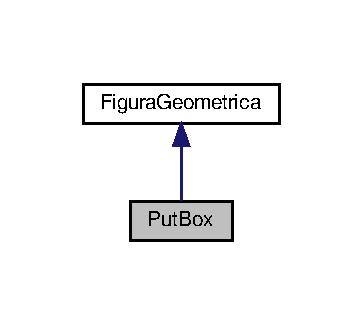
\includegraphics[width=174pt]{class_put_box__inherit__graph}
\end{center}
\end{figure}


Collaboration diagram for Put\+Box\+:
\nopagebreak
\begin{figure}[H]
\begin{center}
\leavevmode
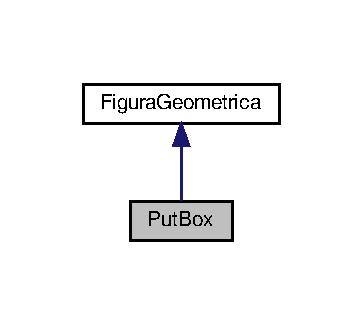
\includegraphics[width=174pt]{class_put_box__coll__graph}
\end{center}
\end{figure}
\subsection*{Public Member Functions}
\begin{DoxyCompactItemize}
\item 
\hyperlink{class_put_box_a0cb7487b6058969a8a015842cf3257de}{Put\+Box} (int x0, int x1, int y0, int y1, int z0, int z1, float \hyperlink{class_figura_geometrica_a0a4f57efb1a6c525c8aeee34c92e7eab}{r}, float \hyperlink{class_figura_geometrica_a51930549bcb90d016b824f10f95df355}{g}, float \hyperlink{class_figura_geometrica_a25e5d6c21410103c25ec55c0117dac0d}{b}, float \hyperlink{class_figura_geometrica_ae7c8a027fcec3c357265b90458a4d165}{a})
\begin{DoxyCompactList}\small\item\em \hyperlink{class_put_box}{Put\+Box} é o construtor da classe, que recebe como parâmetros os valores iniciais e finais das posições nos eixos(x0,x1,y0,y1,z0,z1) e a cor(r,g,b,a) \end{DoxyCompactList}\item 
void \hyperlink{class_put_box_a3caaf01d035f5a0749fd308e9a86de94}{draw} (\hyperlink{class_sculptor}{Sculptor} \&t)
\begin{DoxyCompactList}\small\item\em draw desenha uma caixa para o objeto \hyperlink{class_sculptor}{Sculptor} especificado \end{DoxyCompactList}\end{DoxyCompactItemize}
\subsection*{Additional Inherited Members}


\subsection{Detailed Description}
A classe \hyperlink{class_put_box}{Put\+Box} implementa uma caixa no espaço. 

\subsection{Constructor \& Destructor Documentation}
\mbox{\Hypertarget{class_put_box_a0cb7487b6058969a8a015842cf3257de}\label{class_put_box_a0cb7487b6058969a8a015842cf3257de}} 
\index{Put\+Box@{Put\+Box}!Put\+Box@{Put\+Box}}
\index{Put\+Box@{Put\+Box}!Put\+Box@{Put\+Box}}
\subsubsection{\texorpdfstring{Put\+Box()}{PutBox()}}
{\footnotesize\ttfamily Put\+Box\+::\+Put\+Box (\begin{DoxyParamCaption}\item[{int}]{x0,  }\item[{int}]{x1,  }\item[{int}]{y0,  }\item[{int}]{y1,  }\item[{int}]{z0,  }\item[{int}]{z1,  }\item[{float}]{r,  }\item[{float}]{g,  }\item[{float}]{b,  }\item[{float}]{a }\end{DoxyParamCaption})}



\hyperlink{class_put_box}{Put\+Box} é o construtor da classe, que recebe como parâmetros os valores iniciais e finais das posições nos eixos(x0,x1,y0,y1,z0,z1) e a cor(r,g,b,a) 


\begin{DoxyParams}{Parameters}
{\em x0} & \\
\hline
{\em x1} & \\
\hline
{\em y0} & \\
\hline
{\em y1} & \\
\hline
{\em z0} & \\
\hline
{\em z1} & \\
\hline
{\em r} & \\
\hline
{\em g} & \\
\hline
{\em b} & \\
\hline
{\em a} & \\
\hline
\end{DoxyParams}
exemplo de utilização de \hyperlink{class_put_box}{Put\+Box}\+: 
\begin{DoxyPre}
\hyperlink{class_put_box}{PutBox} pb(1,10,1,10,1,10,1,1,1,1);
\end{DoxyPre}
 

\subsection{Member Function Documentation}
\mbox{\Hypertarget{class_put_box_a3caaf01d035f5a0749fd308e9a86de94}\label{class_put_box_a3caaf01d035f5a0749fd308e9a86de94}} 
\index{Put\+Box@{Put\+Box}!draw@{draw}}
\index{draw@{draw}!Put\+Box@{Put\+Box}}
\subsubsection{\texorpdfstring{draw()}{draw()}}
{\footnotesize\ttfamily void Put\+Box\+::draw (\begin{DoxyParamCaption}\item[{\hyperlink{class_sculptor}{Sculptor} \&}]{t }\end{DoxyParamCaption})\hspace{0.3cm}{\ttfamily [virtual]}}



draw desenha uma caixa para o objeto \hyperlink{class_sculptor}{Sculptor} especificado 


\begin{DoxyParams}{Parameters}
{\em t} & \\
\hline
\end{DoxyParams}


Implements \hyperlink{class_figura_geometrica_a34585fd7c0bd7378fc69c4ee208e676c}{Figura\+Geometrica}.



The documentation for this class was generated from the following files\+:\begin{DoxyCompactItemize}
\item 
\hyperlink{putbox_8h}{putbox.\+h}\item 
\hyperlink{putbox_8cpp}{putbox.\+cpp}\end{DoxyCompactItemize}

\hypertarget{class_put_ellipsoid}{}\section{Put\+Ellipsoid Class Reference}
\label{class_put_ellipsoid}\index{Put\+Ellipsoid@{Put\+Ellipsoid}}


A classe \hyperlink{class_put_ellipsoid}{Put\+Ellipsoid} implementa um elipsoide no espaço.  




{\ttfamily \#include $<$putellipsoid.\+h$>$}



Inheritance diagram for Put\+Ellipsoid\+:
\nopagebreak
\begin{figure}[H]
\begin{center}
\leavevmode
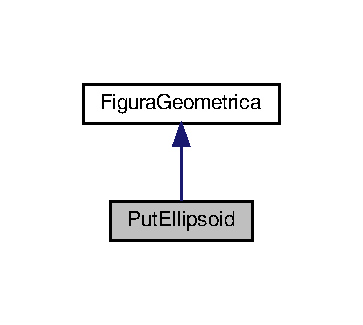
\includegraphics[width=174pt]{class_put_ellipsoid__inherit__graph}
\end{center}
\end{figure}


Collaboration diagram for Put\+Ellipsoid\+:
\nopagebreak
\begin{figure}[H]
\begin{center}
\leavevmode
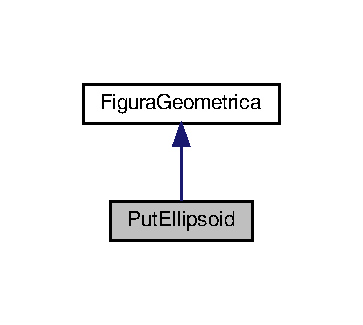
\includegraphics[width=174pt]{class_put_ellipsoid__coll__graph}
\end{center}
\end{figure}
\subsection*{Public Member Functions}
\begin{DoxyCompactItemize}
\item 
\hyperlink{class_put_ellipsoid_a52970ddea7bc1ff99835c06d190383b0}{Put\+Ellipsoid} (int x, int y, int z, int rx, int ry, int rz, float \hyperlink{class_figura_geometrica_a0a4f57efb1a6c525c8aeee34c92e7eab}{r}, float \hyperlink{class_figura_geometrica_a51930549bcb90d016b824f10f95df355}{g}, float \hyperlink{class_figura_geometrica_a25e5d6c21410103c25ec55c0117dac0d}{b}, float \hyperlink{class_figura_geometrica_ae7c8a027fcec3c357265b90458a4d165}{a})
\begin{DoxyCompactList}\small\item\em \hyperlink{class_put_ellipsoid}{Put\+Ellipsoid} é o construtor da classe, que recebe como parâmetros as coordenadas do centro(x,y,z) os raios nos eixos(rx,ry,rz) e a cor(r,g,b,a) \end{DoxyCompactList}\item 
void \hyperlink{class_put_ellipsoid_a961faff306dad93a4b68a35ad9c3027b}{draw} (\hyperlink{class_sculptor}{Sculptor} \&t)
\begin{DoxyCompactList}\small\item\em draw desenha um Elipsoide para o objeto de tipo \hyperlink{class_sculptor}{Sculptor} especificado \end{DoxyCompactList}\end{DoxyCompactItemize}
\subsection*{Additional Inherited Members}


\subsection{Detailed Description}
A classe \hyperlink{class_put_ellipsoid}{Put\+Ellipsoid} implementa um elipsoide no espaço. 

\subsection{Constructor \& Destructor Documentation}
\mbox{\Hypertarget{class_put_ellipsoid_a52970ddea7bc1ff99835c06d190383b0}\label{class_put_ellipsoid_a52970ddea7bc1ff99835c06d190383b0}} 
\index{Put\+Ellipsoid@{Put\+Ellipsoid}!Put\+Ellipsoid@{Put\+Ellipsoid}}
\index{Put\+Ellipsoid@{Put\+Ellipsoid}!Put\+Ellipsoid@{Put\+Ellipsoid}}
\subsubsection{\texorpdfstring{Put\+Ellipsoid()}{PutEllipsoid()}}
{\footnotesize\ttfamily Put\+Ellipsoid\+::\+Put\+Ellipsoid (\begin{DoxyParamCaption}\item[{int}]{x,  }\item[{int}]{y,  }\item[{int}]{z,  }\item[{int}]{rx,  }\item[{int}]{ry,  }\item[{int}]{rz,  }\item[{float}]{r,  }\item[{float}]{g,  }\item[{float}]{b,  }\item[{float}]{a }\end{DoxyParamCaption})}



\hyperlink{class_put_ellipsoid}{Put\+Ellipsoid} é o construtor da classe, que recebe como parâmetros as coordenadas do centro(x,y,z) os raios nos eixos(rx,ry,rz) e a cor(r,g,b,a) 


\begin{DoxyParams}{Parameters}
{\em x} & \\
\hline
{\em y} & \\
\hline
{\em z} & \\
\hline
{\em rx} & \\
\hline
{\em ry} & \\
\hline
{\em rz} & \\
\hline
{\em r} & \\
\hline
{\em g} & \\
\hline
{\em b} & \\
\hline
{\em a} & \\
\hline
\end{DoxyParams}
Exemplo de utilização da classe \hyperlink{class_put_ellipsoid}{Put\+Ellipsoid}\+: 
\begin{DoxyPre}
\hyperlink{class_put_ellipsoid}{PutEllipsoid} pe(10,10,10,2,3,4,1,1,1,1)// Elipsoide centrada em (10,10,10) de raio 2 em,3 em y, 4 em z e cor branca(1,1,1) totalmente opaca(1)
\end{DoxyPre}
 

\subsection{Member Function Documentation}
\mbox{\Hypertarget{class_put_ellipsoid_a961faff306dad93a4b68a35ad9c3027b}\label{class_put_ellipsoid_a961faff306dad93a4b68a35ad9c3027b}} 
\index{Put\+Ellipsoid@{Put\+Ellipsoid}!draw@{draw}}
\index{draw@{draw}!Put\+Ellipsoid@{Put\+Ellipsoid}}
\subsubsection{\texorpdfstring{draw()}{draw()}}
{\footnotesize\ttfamily void Put\+Ellipsoid\+::draw (\begin{DoxyParamCaption}\item[{\hyperlink{class_sculptor}{Sculptor} \&}]{t }\end{DoxyParamCaption})\hspace{0.3cm}{\ttfamily [virtual]}}



draw desenha um Elipsoide para o objeto de tipo \hyperlink{class_sculptor}{Sculptor} especificado 


\begin{DoxyParams}{Parameters}
{\em t} & \\
\hline
\end{DoxyParams}


Implements \hyperlink{class_figura_geometrica_a34585fd7c0bd7378fc69c4ee208e676c}{Figura\+Geometrica}.



The documentation for this class was generated from the following files\+:\begin{DoxyCompactItemize}
\item 
\hyperlink{putellipsoid_8h}{putellipsoid.\+h}\item 
\hyperlink{putellipsoid_8cpp}{putellipsoid.\+cpp}\end{DoxyCompactItemize}

\hypertarget{class_put_sphere}{}\section{Put\+Sphere Class Reference}
\label{class_put_sphere}\index{Put\+Sphere@{Put\+Sphere}}


A classe \hyperlink{class_put_sphere}{Put\+Sphere} implementa uma esfera no espaço.  




{\ttfamily \#include $<$putsphere.\+h$>$}



Inheritance diagram for Put\+Sphere\+:
\nopagebreak
\begin{figure}[H]
\begin{center}
\leavevmode
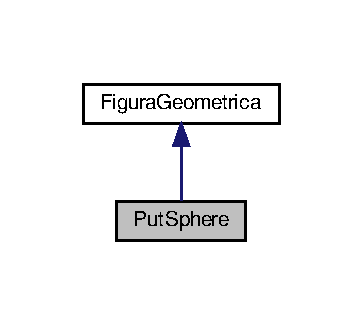
\includegraphics[width=174pt]{class_put_sphere__inherit__graph}
\end{center}
\end{figure}


Collaboration diagram for Put\+Sphere\+:
\nopagebreak
\begin{figure}[H]
\begin{center}
\leavevmode
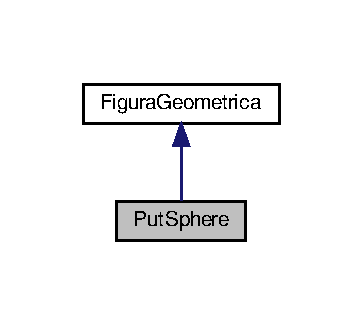
\includegraphics[width=174pt]{class_put_sphere__coll__graph}
\end{center}
\end{figure}
\subsection*{Public Member Functions}
\begin{DoxyCompactItemize}
\item 
\hyperlink{class_put_sphere_a0b70b6e3dba80000008282f38416537c}{Put\+Sphere} (int x, int y, int z, int raio, float \hyperlink{class_figura_geometrica_a0a4f57efb1a6c525c8aeee34c92e7eab}{r}, float \hyperlink{class_figura_geometrica_a51930549bcb90d016b824f10f95df355}{g}, float \hyperlink{class_figura_geometrica_a25e5d6c21410103c25ec55c0117dac0d}{b}, float \hyperlink{class_figura_geometrica_ae7c8a027fcec3c357265b90458a4d165}{a})
\begin{DoxyCompactList}\small\item\em \hyperlink{class_put_sphere}{Put\+Sphere} é o construtor da classe, que recebe como parâmetros as coordenadas do centro da esfera(x,y,z) o tamanho do raio(r) e os parâmetro de cor(r,g,b,a) \end{DoxyCompactList}\item 
void \hyperlink{class_put_sphere_a5105d1e171563e16c148d8f715321b24}{draw} (\hyperlink{class_sculptor}{Sculptor} \&t)
\begin{DoxyCompactList}\small\item\em draw desenha uma esfera para o objeto de tipo \hyperlink{class_sculptor}{Sculptor} especificado \end{DoxyCompactList}\end{DoxyCompactItemize}
\subsection*{Additional Inherited Members}


\subsection{Detailed Description}
A classe \hyperlink{class_put_sphere}{Put\+Sphere} implementa uma esfera no espaço. 

\subsection{Constructor \& Destructor Documentation}
\mbox{\Hypertarget{class_put_sphere_a0b70b6e3dba80000008282f38416537c}\label{class_put_sphere_a0b70b6e3dba80000008282f38416537c}} 
\index{Put\+Sphere@{Put\+Sphere}!Put\+Sphere@{Put\+Sphere}}
\index{Put\+Sphere@{Put\+Sphere}!Put\+Sphere@{Put\+Sphere}}
\subsubsection{\texorpdfstring{Put\+Sphere()}{PutSphere()}}
{\footnotesize\ttfamily Put\+Sphere\+::\+Put\+Sphere (\begin{DoxyParamCaption}\item[{int}]{x,  }\item[{int}]{y,  }\item[{int}]{z,  }\item[{int}]{raio,  }\item[{float}]{r,  }\item[{float}]{g,  }\item[{float}]{b,  }\item[{float}]{a }\end{DoxyParamCaption})}



\hyperlink{class_put_sphere}{Put\+Sphere} é o construtor da classe, que recebe como parâmetros as coordenadas do centro da esfera(x,y,z) o tamanho do raio(r) e os parâmetro de cor(r,g,b,a) 


\begin{DoxyParams}{Parameters}
{\em x} & \\
\hline
{\em y} & \\
\hline
{\em z} & \\
\hline
{\em raio} & \\
\hline
{\em r} & \\
\hline
{\em g} & \\
\hline
{\em b} & \\
\hline
{\em a} & \\
\hline
\end{DoxyParams}
Exemplo de utilização de \hyperlink{class_put_sphere}{Put\+Sphere}\+: A esfera é definida como\+: \[ (X-xc)²+(Y-yc)²+(Z-zc)²=r²\]


\begin{DoxyPre}
\hyperlink{class_put_sphere}{PutSphere} ps(3,3,3,5,1,1,1,1)// esfera centrada em (3,3,3) de raio 5 e cor branca(1,1,1) totalmente opaca(1)
\end{DoxyPre}
 

\subsection{Member Function Documentation}
\mbox{\Hypertarget{class_put_sphere_a5105d1e171563e16c148d8f715321b24}\label{class_put_sphere_a5105d1e171563e16c148d8f715321b24}} 
\index{Put\+Sphere@{Put\+Sphere}!draw@{draw}}
\index{draw@{draw}!Put\+Sphere@{Put\+Sphere}}
\subsubsection{\texorpdfstring{draw()}{draw()}}
{\footnotesize\ttfamily void Put\+Sphere\+::draw (\begin{DoxyParamCaption}\item[{\hyperlink{class_sculptor}{Sculptor} \&}]{t }\end{DoxyParamCaption})\hspace{0.3cm}{\ttfamily [virtual]}}



draw desenha uma esfera para o objeto de tipo \hyperlink{class_sculptor}{Sculptor} especificado 


\begin{DoxyParams}{Parameters}
{\em t} & \\
\hline
\end{DoxyParams}


Implements \hyperlink{class_figura_geometrica_a34585fd7c0bd7378fc69c4ee208e676c}{Figura\+Geometrica}.



The documentation for this class was generated from the following files\+:\begin{DoxyCompactItemize}
\item 
\hyperlink{putsphere_8h}{putsphere.\+h}\item 
\hyperlink{putsphere_8cpp}{putsphere.\+cpp}\end{DoxyCompactItemize}

\hypertarget{class_put_voxel}{}\section{Put\+Voxel Class Reference}
\label{class_put_voxel}\index{Put\+Voxel@{Put\+Voxel}}


A classe \hyperlink{class_put_voxel}{Put\+Voxel} implementa um voxel no espaço.  




{\ttfamily \#include $<$putvoxel.\+h$>$}



Inheritance diagram for Put\+Voxel\+:
\nopagebreak
\begin{figure}[H]
\begin{center}
\leavevmode
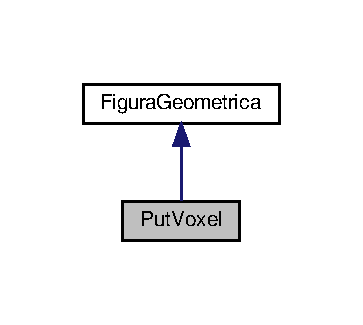
\includegraphics[width=174pt]{class_put_voxel__inherit__graph}
\end{center}
\end{figure}


Collaboration diagram for Put\+Voxel\+:
\nopagebreak
\begin{figure}[H]
\begin{center}
\leavevmode
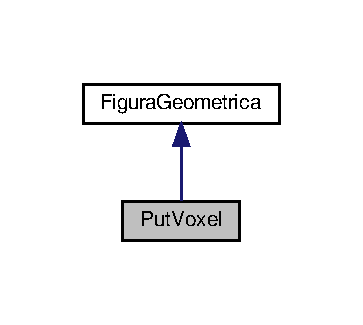
\includegraphics[width=174pt]{class_put_voxel__coll__graph}
\end{center}
\end{figure}
\subsection*{Public Member Functions}
\begin{DoxyCompactItemize}
\item 
\hyperlink{class_put_voxel_aff93a249c1f4919758acd26f34384d05}{Put\+Voxel} (float \hyperlink{class_figura_geometrica_a0a4f57efb1a6c525c8aeee34c92e7eab}{r}, float \hyperlink{class_figura_geometrica_a51930549bcb90d016b824f10f95df355}{g}, float \hyperlink{class_figura_geometrica_a25e5d6c21410103c25ec55c0117dac0d}{b}, float \hyperlink{class_figura_geometrica_ae7c8a027fcec3c357265b90458a4d165}{a}, int x, int y, int z)
\begin{DoxyCompactList}\small\item\em \hyperlink{class_put_voxel}{Put\+Voxel} é o construtor da classe, que recebe como parâmetros os valores da cor(r,g,b,a) e a posição no espaço a qual deseja posicionar. \end{DoxyCompactList}\item 
\hyperlink{class_put_voxel_ac3c14b19e69b462e3178b5dca92d7b34}{$\sim$\+Put\+Voxel} ()
\item 
void \hyperlink{class_put_voxel_af784ab77d8a7aac2010e608796710ccb}{draw} (\hyperlink{class_sculptor}{Sculptor} \&t)
\begin{DoxyCompactList}\small\item\em draw deseha um voxel para o objeto \hyperlink{class_sculptor}{Sculptor} especificado como parâmetro \end{DoxyCompactList}\end{DoxyCompactItemize}
\subsection*{Additional Inherited Members}


\subsection{Detailed Description}
A classe \hyperlink{class_put_voxel}{Put\+Voxel} implementa um voxel no espaço. 

\subsection{Constructor \& Destructor Documentation}
\mbox{\Hypertarget{class_put_voxel_aff93a249c1f4919758acd26f34384d05}\label{class_put_voxel_aff93a249c1f4919758acd26f34384d05}} 
\index{Put\+Voxel@{Put\+Voxel}!Put\+Voxel@{Put\+Voxel}}
\index{Put\+Voxel@{Put\+Voxel}!Put\+Voxel@{Put\+Voxel}}
\subsubsection{\texorpdfstring{Put\+Voxel()}{PutVoxel()}}
{\footnotesize\ttfamily Put\+Voxel\+::\+Put\+Voxel (\begin{DoxyParamCaption}\item[{float}]{r,  }\item[{float}]{g,  }\item[{float}]{b,  }\item[{float}]{a,  }\item[{int}]{x,  }\item[{int}]{y,  }\item[{int}]{z }\end{DoxyParamCaption})}



\hyperlink{class_put_voxel}{Put\+Voxel} é o construtor da classe, que recebe como parâmetros os valores da cor(r,g,b,a) e a posição no espaço a qual deseja posicionar. 


\begin{DoxyParams}{Parameters}
{\em r} & \\
\hline
{\em g} & \\
\hline
{\em b} & \\
\hline
{\em a} & \\
\hline
{\em x} & \\
\hline
{\em y} & \\
\hline
{\em z} & \\
\hline
\end{DoxyParams}
exemplo de declaração de \hyperlink{class_put_voxel}{Put\+Voxel}\+: 
\begin{DoxyPre}
\hyperlink{class_put_voxel}{PutVoxel} pv(1,0,0,1,1,1,1); //cria um voxel de cor vermelha(1,0,0) totalmente opaco na posição (1,1,1)\end{DoxyPre}



\begin{DoxyPre}\end{DoxyPre}
 \mbox{\Hypertarget{class_put_voxel_ac3c14b19e69b462e3178b5dca92d7b34}\label{class_put_voxel_ac3c14b19e69b462e3178b5dca92d7b34}} 
\index{Put\+Voxel@{Put\+Voxel}!````~Put\+Voxel@{$\sim$\+Put\+Voxel}}
\index{````~Put\+Voxel@{$\sim$\+Put\+Voxel}!Put\+Voxel@{Put\+Voxel}}
\subsubsection{\texorpdfstring{$\sim$\+Put\+Voxel()}{~PutVoxel()}}
{\footnotesize\ttfamily Put\+Voxel\+::$\sim$\+Put\+Voxel (\begin{DoxyParamCaption}{ }\end{DoxyParamCaption})}



\subsection{Member Function Documentation}
\mbox{\Hypertarget{class_put_voxel_af784ab77d8a7aac2010e608796710ccb}\label{class_put_voxel_af784ab77d8a7aac2010e608796710ccb}} 
\index{Put\+Voxel@{Put\+Voxel}!draw@{draw}}
\index{draw@{draw}!Put\+Voxel@{Put\+Voxel}}
\subsubsection{\texorpdfstring{draw()}{draw()}}
{\footnotesize\ttfamily void Put\+Voxel\+::draw (\begin{DoxyParamCaption}\item[{\hyperlink{class_sculptor}{Sculptor} \&}]{t }\end{DoxyParamCaption})\hspace{0.3cm}{\ttfamily [virtual]}}



draw deseha um voxel para o objeto \hyperlink{class_sculptor}{Sculptor} especificado como parâmetro 


\begin{DoxyParams}{Parameters}
{\em t} & \\
\hline
\end{DoxyParams}


Implements \hyperlink{class_figura_geometrica_a34585fd7c0bd7378fc69c4ee208e676c}{Figura\+Geometrica}.



The documentation for this class was generated from the following files\+:\begin{DoxyCompactItemize}
\item 
\hyperlink{putvoxel_8h}{putvoxel.\+h}\item 
\hyperlink{putvoxel_8cpp}{putvoxel.\+cpp}\end{DoxyCompactItemize}

\hypertarget{class_sculptor}{}\section{Sculptor Class Reference}
\label{class_sculptor}\index{Sculptor@{Sculptor}}


A classe \hyperlink{class_sculptor}{Sculptor} define o espaço em que os voxels estarão alocados(como se fosse uma \char`\"{}prancheta\char`\"{} de desenho)  




{\ttfamily \#include $<$sculptor.\+h$>$}

\subsection*{Public Member Functions}
\begin{DoxyCompactItemize}
\item 
\hyperlink{class_sculptor_a014e3ef5517bf0e9d9e14486b6ac6433}{Sculptor} (int \+\_\+nx, int \+\_\+ny, int \+\_\+nz)
\begin{DoxyCompactList}\small\item\em \hyperlink{class_sculptor}{Sculptor} é o construtor que recebe como parâmetros os comprimentos em relação aos eixos cartesianos(x,y,z) \end{DoxyCompactList}\item 
\hyperlink{class_sculptor_a8f159bf97458326f16d2e238e11be7ff}{$\sim$\+Sculptor} ()
\begin{DoxyCompactList}\small\item\em $\sim$\+Sculptor é o destrutor da classe \end{DoxyCompactList}\item 
void \hyperlink{class_sculptor_af1d69da01379874b0dfd6454787cb562}{set\+Color} (float r, float g, float b, float alpha)
\begin{DoxyCompactList}\small\item\em set\+Color altera a cor selecionada. \end{DoxyCompactList}\item 
void \hyperlink{class_sculptor_a4bdea3048b419d58e93074060eaa7b52}{put\+Voxel} (int x, int y, int z)
\begin{DoxyCompactList}\small\item\em put\+Voxel Insere um voxel no espaço \end{DoxyCompactList}\item 
void \hyperlink{class_sculptor_ad9d714a35fc8ae16d06eb5df37c3493c}{cut\+Voxel} (int x, int y, int z)
\begin{DoxyCompactList}\small\item\em cut\+Voxel Apaga um voxel no espaço \end{DoxyCompactList}\item 
void \hyperlink{class_sculptor_a311ad7a0fb83fc67ac1f378be8e99fe1}{put\+Box} (int x0, int x1, int y0, int y1, int z0, int z1)
\begin{DoxyCompactList}\small\item\em put\+Box Insere uma caixa no espaço \end{DoxyCompactList}\item 
void \hyperlink{class_sculptor_aa84a1b12b09e9e103fc8d78f8d1bc00f}{cut\+Box} (int x0, int x1, int y0, int y1, int z0, int z1)
\begin{DoxyCompactList}\small\item\em cut\+Box apaga uma caixa do espaço \end{DoxyCompactList}\item 
void \hyperlink{class_sculptor_a7ad429e4c9bee30af79485b97a67885f}{put\+Sphere} (int xc, int yc, int zc, int raio)
\begin{DoxyCompactList}\small\item\em put\+Sphere implementa uma esfera no espaço \end{DoxyCompactList}\item 
void \hyperlink{class_sculptor_a7fc1bd095f9f1019d1619673905f6cdc}{cut\+Sphere} (int xc, int yc, int zc, int raio)
\begin{DoxyCompactList}\small\item\em cut\+Sphere apaga uma esfera no espaço \end{DoxyCompactList}\item 
void \hyperlink{class_sculptor_aab6773c379cee65ef0e93de25079a23d}{put\+Ellipsoid} (int xc, int yc, int zc, int rx, int ry, int rz)
\begin{DoxyCompactList}\small\item\em put\+Ellipsoid implementa um elipsoide no espaço \end{DoxyCompactList}\item 
void \hyperlink{class_sculptor_a84b3495724695476daa2e9b83df7cb03}{cut\+Ellipsoid} (int xc, int yc, int zc, int rx, int ry, int rz)
\begin{DoxyCompactList}\small\item\em cut\+Ellipsoid apaga um elipsoide no espaço \end{DoxyCompactList}\item 
void \hyperlink{class_sculptor_a58cb72d22001a5034f15383ca983830c}{write\+O\+FF} (const char $\ast$filename)
\begin{DoxyCompactList}\small\item\em write\+O\+FF grava a escultura no formato O\+FF no arquivo especificado \end{DoxyCompactList}\item 
bool \hyperlink{class_sculptor_ad7793360e2d6a11c4799b50e3cfaf017}{getisonplan} (int i, int j, int k)
\item 
float \hyperlink{class_sculptor_a6ddea4b268d77d46085313a09746176b}{getR} (int, int, int)
\item 
float \hyperlink{class_sculptor_a82bade484b1942db03407888b0821791}{getG} (int, int, int)
\item 
float \hyperlink{class_sculptor_a101cab6fc879fd4eb756aaa90043805c}{getB} (int, int, int)
\item 
float \hyperlink{class_sculptor_aad4a793c55c48526fb0db2b14a6042cc}{getA} (int, int, int)
\end{DoxyCompactItemize}


\subsection{Detailed Description}
A classe \hyperlink{class_sculptor}{Sculptor} define o espaço em que os voxels estarão alocados(como se fosse uma \char`\"{}prancheta\char`\"{} de desenho) 

\subsection{Constructor \& Destructor Documentation}
\mbox{\Hypertarget{class_sculptor_a014e3ef5517bf0e9d9e14486b6ac6433}\label{class_sculptor_a014e3ef5517bf0e9d9e14486b6ac6433}} 
\index{Sculptor@{Sculptor}!Sculptor@{Sculptor}}
\index{Sculptor@{Sculptor}!Sculptor@{Sculptor}}
\subsubsection{\texorpdfstring{Sculptor()}{Sculptor()}}
{\footnotesize\ttfamily Sculptor\+::\+Sculptor (\begin{DoxyParamCaption}\item[{int}]{\+\_\+nx,  }\item[{int}]{\+\_\+ny,  }\item[{int}]{\+\_\+nz }\end{DoxyParamCaption})}



\hyperlink{class_sculptor}{Sculptor} é o construtor que recebe como parâmetros os comprimentos em relação aos eixos cartesianos(x,y,z) 


\begin{DoxyParams}{Parameters}
{\em \+\_\+nx} & \\
\hline
{\em \+\_\+ny} & \\
\hline
{\em \+\_\+nz} & \\
\hline
\end{DoxyParams}
\mbox{\Hypertarget{class_sculptor_a8f159bf97458326f16d2e238e11be7ff}\label{class_sculptor_a8f159bf97458326f16d2e238e11be7ff}} 
\index{Sculptor@{Sculptor}!````~Sculptor@{$\sim$\+Sculptor}}
\index{````~Sculptor@{$\sim$\+Sculptor}!Sculptor@{Sculptor}}
\subsubsection{\texorpdfstring{$\sim$\+Sculptor()}{~Sculptor()}}
{\footnotesize\ttfamily Sculptor\+::$\sim$\+Sculptor (\begin{DoxyParamCaption}{ }\end{DoxyParamCaption})}



$\sim$\+Sculptor é o destrutor da classe 



\subsection{Member Function Documentation}
\mbox{\Hypertarget{class_sculptor_aa84a1b12b09e9e103fc8d78f8d1bc00f}\label{class_sculptor_aa84a1b12b09e9e103fc8d78f8d1bc00f}} 
\index{Sculptor@{Sculptor}!cut\+Box@{cut\+Box}}
\index{cut\+Box@{cut\+Box}!Sculptor@{Sculptor}}
\subsubsection{\texorpdfstring{cut\+Box()}{cutBox()}}
{\footnotesize\ttfamily void Sculptor\+::cut\+Box (\begin{DoxyParamCaption}\item[{int}]{x0,  }\item[{int}]{x1,  }\item[{int}]{y0,  }\item[{int}]{y1,  }\item[{int}]{z0,  }\item[{int}]{z1 }\end{DoxyParamCaption})}



cut\+Box apaga uma caixa do espaço 


\begin{DoxyParams}{Parameters}
{\em x0} & \\
\hline
{\em x1} & \\
\hline
{\em y0} & \\
\hline
{\em y1} & \\
\hline
{\em z0} & \\
\hline
{\em z1} & \\
\hline
\end{DoxyParams}
\mbox{\Hypertarget{class_sculptor_a84b3495724695476daa2e9b83df7cb03}\label{class_sculptor_a84b3495724695476daa2e9b83df7cb03}} 
\index{Sculptor@{Sculptor}!cut\+Ellipsoid@{cut\+Ellipsoid}}
\index{cut\+Ellipsoid@{cut\+Ellipsoid}!Sculptor@{Sculptor}}
\subsubsection{\texorpdfstring{cut\+Ellipsoid()}{cutEllipsoid()}}
{\footnotesize\ttfamily void Sculptor\+::cut\+Ellipsoid (\begin{DoxyParamCaption}\item[{int}]{xc,  }\item[{int}]{yc,  }\item[{int}]{zc,  }\item[{int}]{rx,  }\item[{int}]{ry,  }\item[{int}]{rz }\end{DoxyParamCaption})}



cut\+Ellipsoid apaga um elipsoide no espaço 


\begin{DoxyParams}{Parameters}
{\em xc} & \\
\hline
{\em yc} & \\
\hline
{\em zc} & \\
\hline
{\em rx} & \\
\hline
{\em ry} & \\
\hline
{\em rz} & \\
\hline
\end{DoxyParams}
\mbox{\Hypertarget{class_sculptor_a7fc1bd095f9f1019d1619673905f6cdc}\label{class_sculptor_a7fc1bd095f9f1019d1619673905f6cdc}} 
\index{Sculptor@{Sculptor}!cut\+Sphere@{cut\+Sphere}}
\index{cut\+Sphere@{cut\+Sphere}!Sculptor@{Sculptor}}
\subsubsection{\texorpdfstring{cut\+Sphere()}{cutSphere()}}
{\footnotesize\ttfamily void Sculptor\+::cut\+Sphere (\begin{DoxyParamCaption}\item[{int}]{xc,  }\item[{int}]{yc,  }\item[{int}]{zc,  }\item[{int}]{raio }\end{DoxyParamCaption})}



cut\+Sphere apaga uma esfera no espaço 


\begin{DoxyParams}{Parameters}
{\em xc} & \\
\hline
{\em yc} & \\
\hline
{\em zc} & \\
\hline
{\em raio} & \\
\hline
\end{DoxyParams}
\mbox{\Hypertarget{class_sculptor_ad9d714a35fc8ae16d06eb5df37c3493c}\label{class_sculptor_ad9d714a35fc8ae16d06eb5df37c3493c}} 
\index{Sculptor@{Sculptor}!cut\+Voxel@{cut\+Voxel}}
\index{cut\+Voxel@{cut\+Voxel}!Sculptor@{Sculptor}}
\subsubsection{\texorpdfstring{cut\+Voxel()}{cutVoxel()}}
{\footnotesize\ttfamily void Sculptor\+::cut\+Voxel (\begin{DoxyParamCaption}\item[{int}]{x,  }\item[{int}]{y,  }\item[{int}]{z }\end{DoxyParamCaption})}



cut\+Voxel Apaga um voxel no espaço 


\begin{DoxyParams}{Parameters}
{\em x} & \\
\hline
{\em y} & \\
\hline
{\em z} & \\
\hline
\end{DoxyParams}
\mbox{\Hypertarget{class_sculptor_aad4a793c55c48526fb0db2b14a6042cc}\label{class_sculptor_aad4a793c55c48526fb0db2b14a6042cc}} 
\index{Sculptor@{Sculptor}!getA@{getA}}
\index{getA@{getA}!Sculptor@{Sculptor}}
\subsubsection{\texorpdfstring{get\+A()}{getA()}}
{\footnotesize\ttfamily float Sculptor\+::getA (\begin{DoxyParamCaption}\item[{int}]{i,  }\item[{int}]{j,  }\item[{int}]{k }\end{DoxyParamCaption})}

\mbox{\Hypertarget{class_sculptor_a101cab6fc879fd4eb756aaa90043805c}\label{class_sculptor_a101cab6fc879fd4eb756aaa90043805c}} 
\index{Sculptor@{Sculptor}!getB@{getB}}
\index{getB@{getB}!Sculptor@{Sculptor}}
\subsubsection{\texorpdfstring{get\+B()}{getB()}}
{\footnotesize\ttfamily float Sculptor\+::getB (\begin{DoxyParamCaption}\item[{int}]{i,  }\item[{int}]{j,  }\item[{int}]{k }\end{DoxyParamCaption})}

\mbox{\Hypertarget{class_sculptor_a82bade484b1942db03407888b0821791}\label{class_sculptor_a82bade484b1942db03407888b0821791}} 
\index{Sculptor@{Sculptor}!getG@{getG}}
\index{getG@{getG}!Sculptor@{Sculptor}}
\subsubsection{\texorpdfstring{get\+G()}{getG()}}
{\footnotesize\ttfamily float Sculptor\+::getG (\begin{DoxyParamCaption}\item[{int}]{i,  }\item[{int}]{j,  }\item[{int}]{k }\end{DoxyParamCaption})}

\mbox{\Hypertarget{class_sculptor_ad7793360e2d6a11c4799b50e3cfaf017}\label{class_sculptor_ad7793360e2d6a11c4799b50e3cfaf017}} 
\index{Sculptor@{Sculptor}!getisonplan@{getisonplan}}
\index{getisonplan@{getisonplan}!Sculptor@{Sculptor}}
\subsubsection{\texorpdfstring{getisonplan()}{getisonplan()}}
{\footnotesize\ttfamily bool Sculptor\+::getisonplan (\begin{DoxyParamCaption}\item[{int}]{i,  }\item[{int}]{j,  }\item[{int}]{k }\end{DoxyParamCaption})}

\mbox{\Hypertarget{class_sculptor_a6ddea4b268d77d46085313a09746176b}\label{class_sculptor_a6ddea4b268d77d46085313a09746176b}} 
\index{Sculptor@{Sculptor}!getR@{getR}}
\index{getR@{getR}!Sculptor@{Sculptor}}
\subsubsection{\texorpdfstring{get\+R()}{getR()}}
{\footnotesize\ttfamily float Sculptor\+::getR (\begin{DoxyParamCaption}\item[{int}]{i,  }\item[{int}]{j,  }\item[{int}]{k }\end{DoxyParamCaption})}

\mbox{\Hypertarget{class_sculptor_a311ad7a0fb83fc67ac1f378be8e99fe1}\label{class_sculptor_a311ad7a0fb83fc67ac1f378be8e99fe1}} 
\index{Sculptor@{Sculptor}!put\+Box@{put\+Box}}
\index{put\+Box@{put\+Box}!Sculptor@{Sculptor}}
\subsubsection{\texorpdfstring{put\+Box()}{putBox()}}
{\footnotesize\ttfamily void Sculptor\+::put\+Box (\begin{DoxyParamCaption}\item[{int}]{x0,  }\item[{int}]{x1,  }\item[{int}]{y0,  }\item[{int}]{y1,  }\item[{int}]{z0,  }\item[{int}]{z1 }\end{DoxyParamCaption})}



put\+Box Insere uma caixa no espaço 


\begin{DoxyParams}{Parameters}
{\em x0} & \\
\hline
{\em x1} & \\
\hline
{\em y0} & \\
\hline
{\em y1} & \\
\hline
{\em z0} & \\
\hline
{\em z1} & \\
\hline
\end{DoxyParams}
\mbox{\Hypertarget{class_sculptor_aab6773c379cee65ef0e93de25079a23d}\label{class_sculptor_aab6773c379cee65ef0e93de25079a23d}} 
\index{Sculptor@{Sculptor}!put\+Ellipsoid@{put\+Ellipsoid}}
\index{put\+Ellipsoid@{put\+Ellipsoid}!Sculptor@{Sculptor}}
\subsubsection{\texorpdfstring{put\+Ellipsoid()}{putEllipsoid()}}
{\footnotesize\ttfamily void Sculptor\+::put\+Ellipsoid (\begin{DoxyParamCaption}\item[{int}]{xc,  }\item[{int}]{yc,  }\item[{int}]{zc,  }\item[{int}]{rx,  }\item[{int}]{ry,  }\item[{int}]{rz }\end{DoxyParamCaption})}



put\+Ellipsoid implementa um elipsoide no espaço 


\begin{DoxyParams}{Parameters}
{\em xc} & \\
\hline
{\em yc} & \\
\hline
{\em zc} & \\
\hline
{\em rx} & \\
\hline
{\em ry} & \\
\hline
{\em rz} & \\
\hline
\end{DoxyParams}
\mbox{\Hypertarget{class_sculptor_a7ad429e4c9bee30af79485b97a67885f}\label{class_sculptor_a7ad429e4c9bee30af79485b97a67885f}} 
\index{Sculptor@{Sculptor}!put\+Sphere@{put\+Sphere}}
\index{put\+Sphere@{put\+Sphere}!Sculptor@{Sculptor}}
\subsubsection{\texorpdfstring{put\+Sphere()}{putSphere()}}
{\footnotesize\ttfamily void Sculptor\+::put\+Sphere (\begin{DoxyParamCaption}\item[{int}]{xc,  }\item[{int}]{yc,  }\item[{int}]{zc,  }\item[{int}]{raio }\end{DoxyParamCaption})}



put\+Sphere implementa uma esfera no espaço 


\begin{DoxyParams}{Parameters}
{\em xc} & \\
\hline
{\em yc} & \\
\hline
{\em zc} & \\
\hline
{\em raio} & \\
\hline
\end{DoxyParams}
\mbox{\Hypertarget{class_sculptor_a4bdea3048b419d58e93074060eaa7b52}\label{class_sculptor_a4bdea3048b419d58e93074060eaa7b52}} 
\index{Sculptor@{Sculptor}!put\+Voxel@{put\+Voxel}}
\index{put\+Voxel@{put\+Voxel}!Sculptor@{Sculptor}}
\subsubsection{\texorpdfstring{put\+Voxel()}{putVoxel()}}
{\footnotesize\ttfamily void Sculptor\+::put\+Voxel (\begin{DoxyParamCaption}\item[{int}]{x,  }\item[{int}]{y,  }\item[{int}]{z }\end{DoxyParamCaption})}



put\+Voxel Insere um voxel no espaço 


\begin{DoxyParams}{Parameters}
{\em x} & \\
\hline
{\em y} & \\
\hline
{\em z} & \\
\hline
\end{DoxyParams}
\mbox{\Hypertarget{class_sculptor_af1d69da01379874b0dfd6454787cb562}\label{class_sculptor_af1d69da01379874b0dfd6454787cb562}} 
\index{Sculptor@{Sculptor}!set\+Color@{set\+Color}}
\index{set\+Color@{set\+Color}!Sculptor@{Sculptor}}
\subsubsection{\texorpdfstring{set\+Color()}{setColor()}}
{\footnotesize\ttfamily void Sculptor\+::set\+Color (\begin{DoxyParamCaption}\item[{float}]{r,  }\item[{float}]{g,  }\item[{float}]{b,  }\item[{float}]{alpha }\end{DoxyParamCaption})}



set\+Color altera a cor selecionada. 


\begin{DoxyParams}{Parameters}
{\em r} & \\
\hline
{\em g} & \\
\hline
{\em b} & \\
\hline
{\em alpha} & \\
\hline
\end{DoxyParams}
\mbox{\Hypertarget{class_sculptor_a58cb72d22001a5034f15383ca983830c}\label{class_sculptor_a58cb72d22001a5034f15383ca983830c}} 
\index{Sculptor@{Sculptor}!write\+O\+FF@{write\+O\+FF}}
\index{write\+O\+FF@{write\+O\+FF}!Sculptor@{Sculptor}}
\subsubsection{\texorpdfstring{write\+O\+F\+F()}{writeOFF()}}
{\footnotesize\ttfamily void Sculptor\+::write\+O\+FF (\begin{DoxyParamCaption}\item[{const char $\ast$}]{filename }\end{DoxyParamCaption})}



write\+O\+FF grava a escultura no formato O\+FF no arquivo especificado 


\begin{DoxyParams}{Parameters}
{\em filename} & \\
\hline
\end{DoxyParams}


The documentation for this class was generated from the following files\+:\begin{DoxyCompactItemize}
\item 
\hyperlink{sculptor_8h}{sculptor.\+h}\item 
\hyperlink{_sculptor_8cpp}{Sculptor.\+cpp}\end{DoxyCompactItemize}

\hypertarget{class_sphere_dialog}{}\section{Sphere\+Dialog Class Reference}
\label{class_sphere_dialog}\index{Sphere\+Dialog@{Sphere\+Dialog}}


{\ttfamily \#include $<$spheredialog.\+h$>$}



Inheritance diagram for Sphere\+Dialog\+:
\nopagebreak
\begin{figure}[H]
\begin{center}
\leavevmode
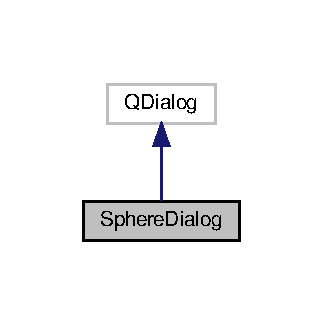
\includegraphics[width=155pt]{class_sphere_dialog__inherit__graph}
\end{center}
\end{figure}


Collaboration diagram for Sphere\+Dialog\+:
\nopagebreak
\begin{figure}[H]
\begin{center}
\leavevmode
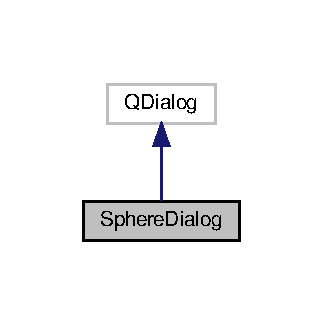
\includegraphics[width=155pt]{class_sphere_dialog__coll__graph}
\end{center}
\end{figure}
\subsection*{Public Member Functions}
\begin{DoxyCompactItemize}
\item 
\hyperlink{class_sphere_dialog_a27970d61eb4311914b22aa3cb22e9750}{Sphere\+Dialog} (Q\+Widget $\ast$parent=nullptr)
\item 
\hyperlink{class_sphere_dialog_aaf6160cf0bb93b2a044b471f34e650ea}{$\sim$\+Sphere\+Dialog} ()
\item 
int \hyperlink{class_sphere_dialog_af78dddeb66fb74be6e749a94c3b81fb3}{get\+Radius} ()
\end{DoxyCompactItemize}


\subsection{Constructor \& Destructor Documentation}
\mbox{\Hypertarget{class_sphere_dialog_a27970d61eb4311914b22aa3cb22e9750}\label{class_sphere_dialog_a27970d61eb4311914b22aa3cb22e9750}} 
\index{Sphere\+Dialog@{Sphere\+Dialog}!Sphere\+Dialog@{Sphere\+Dialog}}
\index{Sphere\+Dialog@{Sphere\+Dialog}!Sphere\+Dialog@{Sphere\+Dialog}}
\subsubsection{\texorpdfstring{Sphere\+Dialog()}{SphereDialog()}}
{\footnotesize\ttfamily Sphere\+Dialog\+::\+Sphere\+Dialog (\begin{DoxyParamCaption}\item[{Q\+Widget $\ast$}]{parent = {\ttfamily nullptr} }\end{DoxyParamCaption})\hspace{0.3cm}{\ttfamily [explicit]}}

\mbox{\Hypertarget{class_sphere_dialog_aaf6160cf0bb93b2a044b471f34e650ea}\label{class_sphere_dialog_aaf6160cf0bb93b2a044b471f34e650ea}} 
\index{Sphere\+Dialog@{Sphere\+Dialog}!````~Sphere\+Dialog@{$\sim$\+Sphere\+Dialog}}
\index{````~Sphere\+Dialog@{$\sim$\+Sphere\+Dialog}!Sphere\+Dialog@{Sphere\+Dialog}}
\subsubsection{\texorpdfstring{$\sim$\+Sphere\+Dialog()}{~SphereDialog()}}
{\footnotesize\ttfamily Sphere\+Dialog\+::$\sim$\+Sphere\+Dialog (\begin{DoxyParamCaption}{ }\end{DoxyParamCaption})}



\subsection{Member Function Documentation}
\mbox{\Hypertarget{class_sphere_dialog_af78dddeb66fb74be6e749a94c3b81fb3}\label{class_sphere_dialog_af78dddeb66fb74be6e749a94c3b81fb3}} 
\index{Sphere\+Dialog@{Sphere\+Dialog}!get\+Radius@{get\+Radius}}
\index{get\+Radius@{get\+Radius}!Sphere\+Dialog@{Sphere\+Dialog}}
\subsubsection{\texorpdfstring{get\+Radius()}{getRadius()}}
{\footnotesize\ttfamily int Sphere\+Dialog\+::get\+Radius (\begin{DoxyParamCaption}{ }\end{DoxyParamCaption})}



The documentation for this class was generated from the following files\+:\begin{DoxyCompactItemize}
\item 
\hyperlink{spheredialog_8h}{spheredialog.\+h}\item 
\hyperlink{spheredialog_8cpp}{spheredialog.\+cpp}\end{DoxyCompactItemize}

\hypertarget{struct_voxel}{}\section{Voxel Struct Reference}
\label{struct_voxel}\index{Voxel@{Voxel}}


O \hyperlink{struct_voxel}{Voxel} consiste em um cubo localizado no espaço tridimensional que possui cor, transparência e pode ou não estar ativado.  




{\ttfamily \#include $<$sculptor.\+h$>$}

\subsection*{Public Attributes}
\begin{DoxyCompactItemize}
\item 
float \hyperlink{struct_voxel_a06872ec79b836120b551a848968c0f1b}{r}
\item 
float \hyperlink{struct_voxel_a27c0da1ed2ff430401d23ff171612a73}{g}
\item 
float \hyperlink{struct_voxel_a5cd8432b1d7d0fd8b79e0fc7d10373a8}{b}
\item 
float \hyperlink{struct_voxel_a3ce2579eb0a9f09a07112ce7498a638e}{a}
\item 
bool \hyperlink{struct_voxel_a6fbe8bd53f64685ac4210726d40fc775}{is\+On}
\end{DoxyCompactItemize}


\subsection{Detailed Description}
O \hyperlink{struct_voxel}{Voxel} consiste em um cubo localizado no espaço tridimensional que possui cor, transparência e pode ou não estar ativado. 

\subsection{Member Data Documentation}
\mbox{\Hypertarget{struct_voxel_a3ce2579eb0a9f09a07112ce7498a638e}\label{struct_voxel_a3ce2579eb0a9f09a07112ce7498a638e}} 
\index{Voxel@{Voxel}!a@{a}}
\index{a@{a}!Voxel@{Voxel}}
\subsubsection{\texorpdfstring{a}{a}}
{\footnotesize\ttfamily float Voxel\+::a}

\mbox{\Hypertarget{struct_voxel_a5cd8432b1d7d0fd8b79e0fc7d10373a8}\label{struct_voxel_a5cd8432b1d7d0fd8b79e0fc7d10373a8}} 
\index{Voxel@{Voxel}!b@{b}}
\index{b@{b}!Voxel@{Voxel}}
\subsubsection{\texorpdfstring{b}{b}}
{\footnotesize\ttfamily float Voxel\+::b}

\mbox{\Hypertarget{struct_voxel_a27c0da1ed2ff430401d23ff171612a73}\label{struct_voxel_a27c0da1ed2ff430401d23ff171612a73}} 
\index{Voxel@{Voxel}!g@{g}}
\index{g@{g}!Voxel@{Voxel}}
\subsubsection{\texorpdfstring{g}{g}}
{\footnotesize\ttfamily float Voxel\+::g}

\mbox{\Hypertarget{struct_voxel_a6fbe8bd53f64685ac4210726d40fc775}\label{struct_voxel_a6fbe8bd53f64685ac4210726d40fc775}} 
\index{Voxel@{Voxel}!is\+On@{is\+On}}
\index{is\+On@{is\+On}!Voxel@{Voxel}}
\subsubsection{\texorpdfstring{is\+On}{isOn}}
{\footnotesize\ttfamily bool Voxel\+::is\+On}

\mbox{\Hypertarget{struct_voxel_a06872ec79b836120b551a848968c0f1b}\label{struct_voxel_a06872ec79b836120b551a848968c0f1b}} 
\index{Voxel@{Voxel}!r@{r}}
\index{r@{r}!Voxel@{Voxel}}
\subsubsection{\texorpdfstring{r}{r}}
{\footnotesize\ttfamily float Voxel\+::r}



The documentation for this struct was generated from the following file\+:\begin{DoxyCompactItemize}
\item 
\hyperlink{sculptor_8h}{sculptor.\+h}\end{DoxyCompactItemize}

\chapter{File Documentation}
\hypertarget{boxdialog_8cpp}{}\section{boxdialog.\+cpp File Reference}
\label{boxdialog_8cpp}\index{boxdialog.\+cpp@{boxdialog.\+cpp}}
{\ttfamily \#include \char`\"{}boxdialog.\+h\char`\"{}}\newline
{\ttfamily \#include \char`\"{}ui\+\_\+boxdialog.\+h\char`\"{}}\newline
Include dependency graph for boxdialog.\+cpp\+:
\nopagebreak
\begin{figure}[H]
\begin{center}
\leavevmode
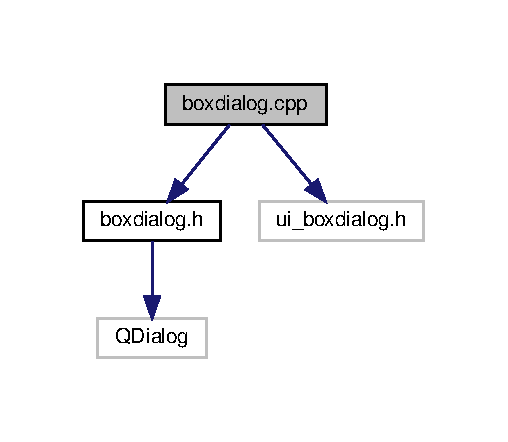
\includegraphics[width=244pt]{boxdialog_8cpp__incl}
\end{center}
\end{figure}

\hypertarget{boxdialog_8h}{}\section{boxdialog.\+h File Reference}
\label{boxdialog_8h}\index{boxdialog.\+h@{boxdialog.\+h}}
{\ttfamily \#include $<$Q\+Dialog$>$}\newline
Include dependency graph for boxdialog.\+h\+:
\nopagebreak
\begin{figure}[H]
\begin{center}
\leavevmode
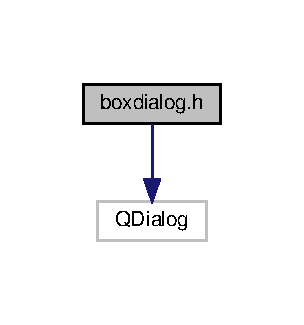
\includegraphics[width=146pt]{boxdialog_8h__incl}
\end{center}
\end{figure}
This graph shows which files directly or indirectly include this file\+:
\nopagebreak
\begin{figure}[H]
\begin{center}
\leavevmode
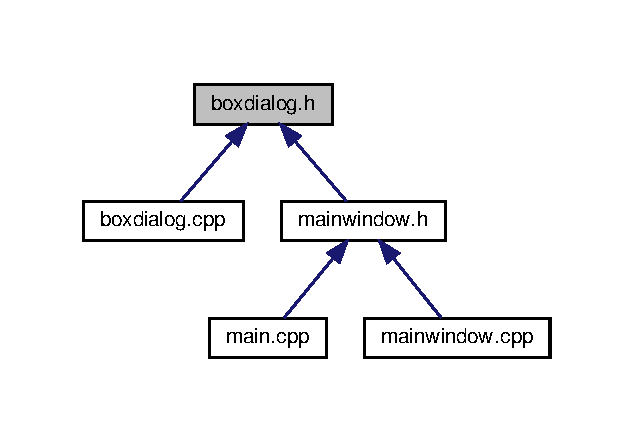
\includegraphics[width=304pt]{boxdialog_8h__dep__incl}
\end{center}
\end{figure}
\subsection*{Classes}
\begin{DoxyCompactItemize}
\item 
class \hyperlink{classbox_dialog}{box\+Dialog}
\end{DoxyCompactItemize}
\subsection*{Namespaces}
\begin{DoxyCompactItemize}
\item 
 \hyperlink{namespace_ui}{Ui}
\end{DoxyCompactItemize}

\hypertarget{cutbox_8cpp}{}\section{cutbox.\+cpp File Reference}
\label{cutbox_8cpp}\index{cutbox.\+cpp@{cutbox.\+cpp}}
{\ttfamily \#include \char`\"{}cutbox.\+h\char`\"{}}\newline
Include dependency graph for cutbox.\+cpp\+:
\nopagebreak
\begin{figure}[H]
\begin{center}
\leavevmode
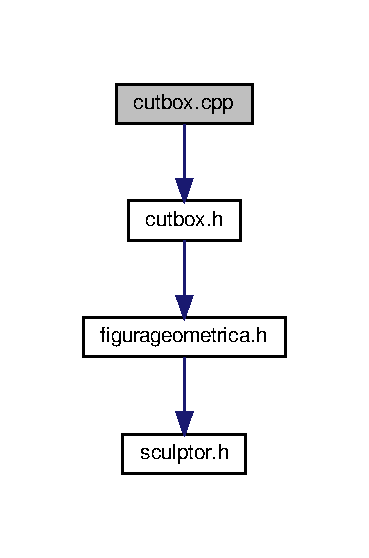
\includegraphics[width=177pt]{cutbox_8cpp__incl}
\end{center}
\end{figure}

\hypertarget{cutbox_8h}{}\section{cutbox.\+h File Reference}
\label{cutbox_8h}\index{cutbox.\+h@{cutbox.\+h}}
{\ttfamily \#include \char`\"{}figurageometrica.\+h\char`\"{}}\newline
Include dependency graph for cutbox.\+h\+:
\nopagebreak
\begin{figure}[H]
\begin{center}
\leavevmode
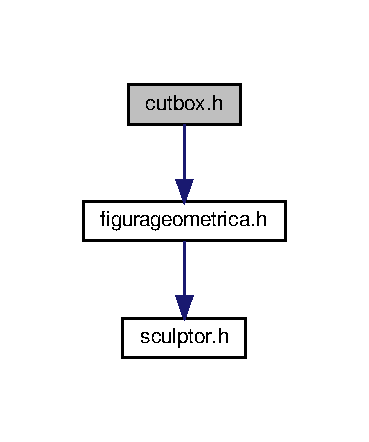
\includegraphics[width=177pt]{cutbox_8h__incl}
\end{center}
\end{figure}
This graph shows which files directly or indirectly include this file\+:
\nopagebreak
\begin{figure}[H]
\begin{center}
\leavevmode
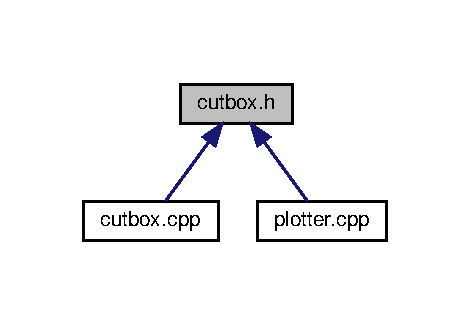
\includegraphics[width=226pt]{cutbox_8h__dep__incl}
\end{center}
\end{figure}
\subsection*{Classes}
\begin{DoxyCompactItemize}
\item 
class \hyperlink{class_cut_box}{Cut\+Box}
\begin{DoxyCompactList}\small\item\em A classe \hyperlink{class_cut_box}{Cut\+Box} apaga uma caixa no espaço. \end{DoxyCompactList}\end{DoxyCompactItemize}

\hypertarget{cutellipsoid_8cpp}{}\section{cutellipsoid.\+cpp File Reference}
\label{cutellipsoid_8cpp}\index{cutellipsoid.\+cpp@{cutellipsoid.\+cpp}}
{\ttfamily \#include \char`\"{}cutellipsoid.\+h\char`\"{}}\newline
Include dependency graph for cutellipsoid.\+cpp\+:
\nopagebreak
\begin{figure}[H]
\begin{center}
\leavevmode
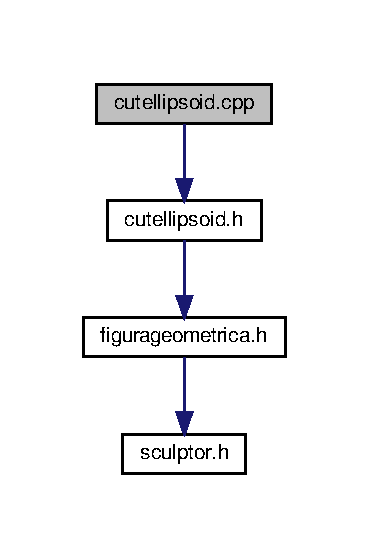
\includegraphics[width=177pt]{cutellipsoid_8cpp__incl}
\end{center}
\end{figure}

\hypertarget{cutellipsoid_8h}{}\section{cutellipsoid.\+h File Reference}
\label{cutellipsoid_8h}\index{cutellipsoid.\+h@{cutellipsoid.\+h}}
{\ttfamily \#include \char`\"{}figurageometrica.\+h\char`\"{}}\newline
Include dependency graph for cutellipsoid.\+h\+:
\nopagebreak
\begin{figure}[H]
\begin{center}
\leavevmode
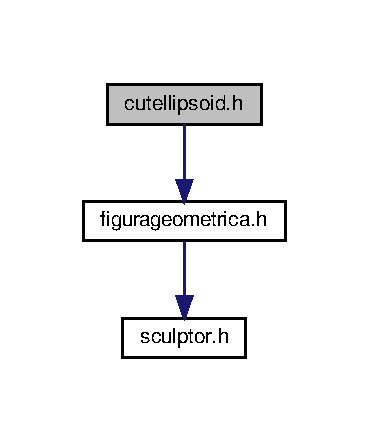
\includegraphics[width=177pt]{cutellipsoid_8h__incl}
\end{center}
\end{figure}
This graph shows which files directly or indirectly include this file\+:
\nopagebreak
\begin{figure}[H]
\begin{center}
\leavevmode
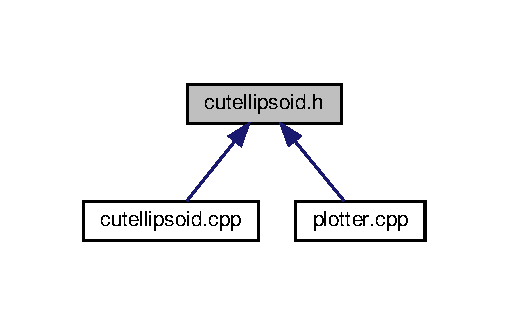
\includegraphics[width=244pt]{cutellipsoid_8h__dep__incl}
\end{center}
\end{figure}
\subsection*{Classes}
\begin{DoxyCompactItemize}
\item 
class \hyperlink{class_cut_ellipsoid}{Cut\+Ellipsoid}
\begin{DoxyCompactList}\small\item\em A classe \hyperlink{class_cut_ellipsoid}{Cut\+Ellipsoid} apaga um elipsoide no espaço. \end{DoxyCompactList}\end{DoxyCompactItemize}

\hypertarget{cutsphere_8cpp}{}\section{cutsphere.\+cpp File Reference}
\label{cutsphere_8cpp}\index{cutsphere.\+cpp@{cutsphere.\+cpp}}
{\ttfamily \#include \char`\"{}cutsphere.\+h\char`\"{}}\newline
Include dependency graph for cutsphere.\+cpp\+:
\nopagebreak
\begin{figure}[H]
\begin{center}
\leavevmode
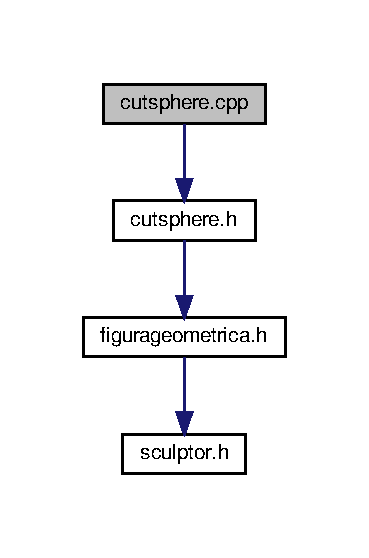
\includegraphics[width=177pt]{cutsphere_8cpp__incl}
\end{center}
\end{figure}

\hypertarget{cutsphere_8h}{}\section{cutsphere.\+h File Reference}
\label{cutsphere_8h}\index{cutsphere.\+h@{cutsphere.\+h}}
{\ttfamily \#include \char`\"{}figurageometrica.\+h\char`\"{}}\newline
Include dependency graph for cutsphere.\+h\+:
\nopagebreak
\begin{figure}[H]
\begin{center}
\leavevmode
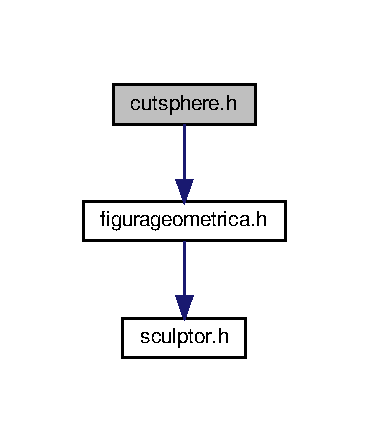
\includegraphics[width=177pt]{cutsphere_8h__incl}
\end{center}
\end{figure}
This graph shows which files directly or indirectly include this file\+:
\nopagebreak
\begin{figure}[H]
\begin{center}
\leavevmode
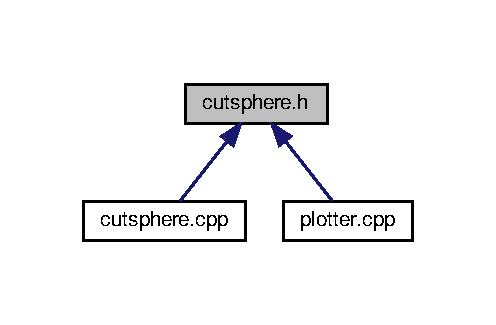
\includegraphics[width=238pt]{cutsphere_8h__dep__incl}
\end{center}
\end{figure}
\subsection*{Classes}
\begin{DoxyCompactItemize}
\item 
class \hyperlink{class_cut_sphere}{Cut\+Sphere}
\begin{DoxyCompactList}\small\item\em A classe \hyperlink{class_cut_sphere}{Cut\+Sphere} apaga uma esfera no espaço. \end{DoxyCompactList}\end{DoxyCompactItemize}

\hypertarget{cutvoxel_8cpp}{}\section{cutvoxel.\+cpp File Reference}
\label{cutvoxel_8cpp}\index{cutvoxel.\+cpp@{cutvoxel.\+cpp}}
{\ttfamily \#include \char`\"{}cutvoxel.\+h\char`\"{}}\newline
Include dependency graph for cutvoxel.\+cpp\+:
\nopagebreak
\begin{figure}[H]
\begin{center}
\leavevmode
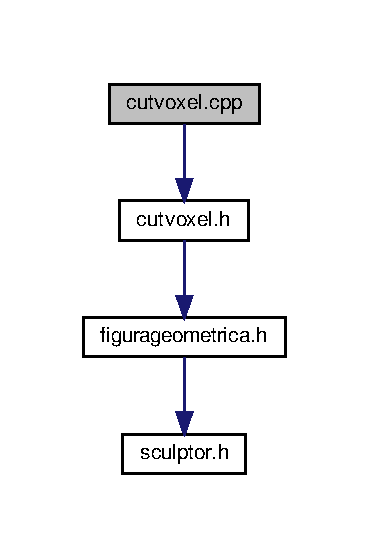
\includegraphics[width=177pt]{cutvoxel_8cpp__incl}
\end{center}
\end{figure}

\hypertarget{cutvoxel_8h}{}\section{cutvoxel.\+h File Reference}
\label{cutvoxel_8h}\index{cutvoxel.\+h@{cutvoxel.\+h}}
{\ttfamily \#include \char`\"{}figurageometrica.\+h\char`\"{}}\newline
Include dependency graph for cutvoxel.\+h\+:
\nopagebreak
\begin{figure}[H]
\begin{center}
\leavevmode
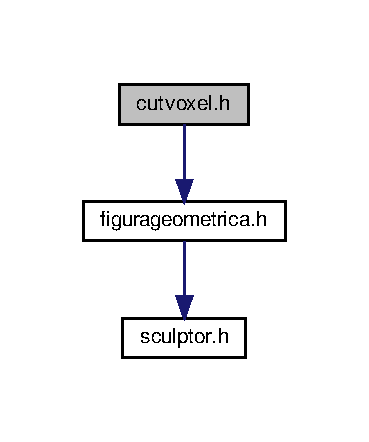
\includegraphics[width=177pt]{cutvoxel_8h__incl}
\end{center}
\end{figure}
This graph shows which files directly or indirectly include this file\+:
\nopagebreak
\begin{figure}[H]
\begin{center}
\leavevmode
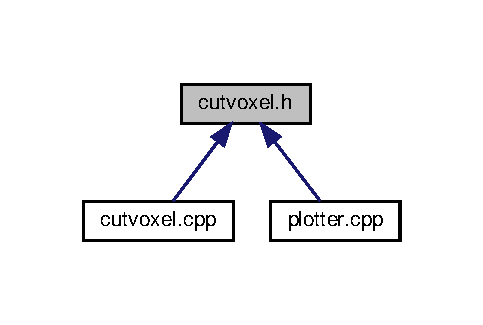
\includegraphics[width=232pt]{cutvoxel_8h__dep__incl}
\end{center}
\end{figure}
\subsection*{Classes}
\begin{DoxyCompactItemize}
\item 
class \hyperlink{class_cut_voxel}{Cut\+Voxel}
\begin{DoxyCompactList}\small\item\em A classe \hyperlink{class_cut_voxel}{Cut\+Voxel} apaga um voxel na posição especificada. \end{DoxyCompactList}\end{DoxyCompactItemize}

\hypertarget{dimdialog_8cpp}{}\section{dimdialog.\+cpp File Reference}
\label{dimdialog_8cpp}\index{dimdialog.\+cpp@{dimdialog.\+cpp}}
{\ttfamily \#include \char`\"{}dimdialog.\+h\char`\"{}}\newline
{\ttfamily \#include \char`\"{}ui\+\_\+dimdialog.\+h\char`\"{}}\newline
Include dependency graph for dimdialog.\+cpp\+:
\nopagebreak
\begin{figure}[H]
\begin{center}
\leavevmode
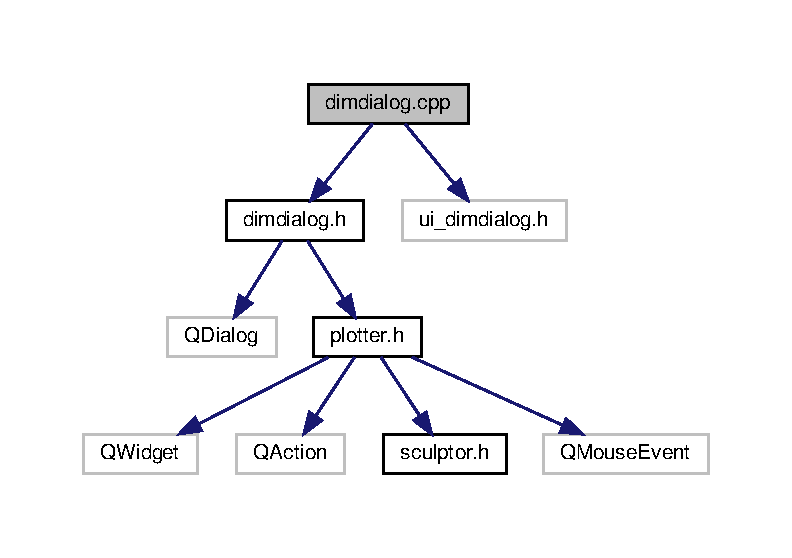
\includegraphics[width=350pt]{dimdialog_8cpp__incl}
\end{center}
\end{figure}

\hypertarget{dimdialog_8h}{}\section{dimdialog.\+h File Reference}
\label{dimdialog_8h}\index{dimdialog.\+h@{dimdialog.\+h}}
{\ttfamily \#include $<$Q\+Dialog$>$}\newline
{\ttfamily \#include $<$plotter.\+h$>$}\newline
Include dependency graph for dimdialog.\+h\+:
\nopagebreak
\begin{figure}[H]
\begin{center}
\leavevmode
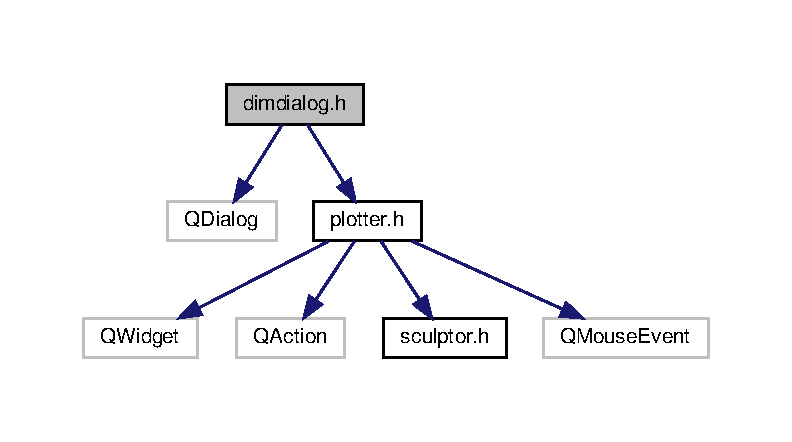
\includegraphics[width=350pt]{dimdialog_8h__incl}
\end{center}
\end{figure}
This graph shows which files directly or indirectly include this file\+:
\nopagebreak
\begin{figure}[H]
\begin{center}
\leavevmode
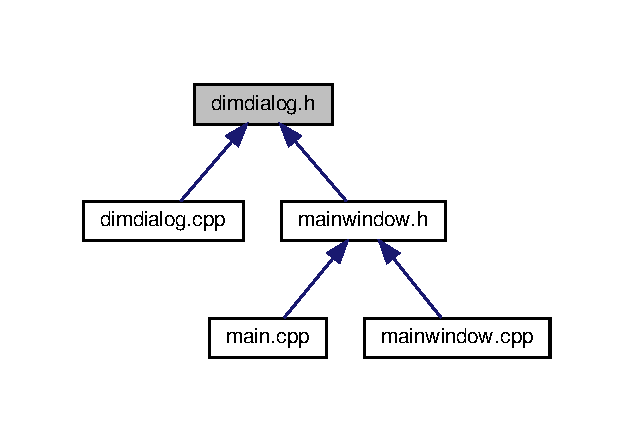
\includegraphics[width=304pt]{dimdialog_8h__dep__incl}
\end{center}
\end{figure}
\subsection*{Classes}
\begin{DoxyCompactItemize}
\item 
class \hyperlink{classdim_dialog}{dim\+Dialog}
\end{DoxyCompactItemize}
\subsection*{Namespaces}
\begin{DoxyCompactItemize}
\item 
 \hyperlink{namespace_ui}{Ui}
\end{DoxyCompactItemize}

\hypertarget{ellipsoiddialog_8cpp}{}\section{ellipsoiddialog.\+cpp File Reference}
\label{ellipsoiddialog_8cpp}\index{ellipsoiddialog.\+cpp@{ellipsoiddialog.\+cpp}}
{\ttfamily \#include \char`\"{}ellipsoiddialog.\+h\char`\"{}}\newline
{\ttfamily \#include \char`\"{}ui\+\_\+ellipsoiddialog.\+h\char`\"{}}\newline
Include dependency graph for ellipsoiddialog.\+cpp\+:
\nopagebreak
\begin{figure}[H]
\begin{center}
\leavevmode
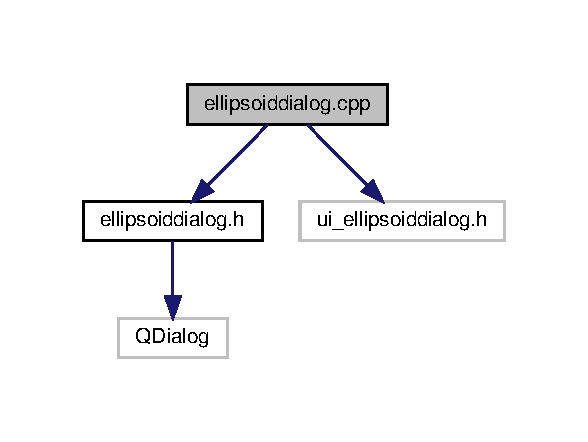
\includegraphics[width=282pt]{ellipsoiddialog_8cpp__incl}
\end{center}
\end{figure}

\hypertarget{ellipsoiddialog_8h}{}\section{ellipsoiddialog.\+h File Reference}
\label{ellipsoiddialog_8h}\index{ellipsoiddialog.\+h@{ellipsoiddialog.\+h}}
{\ttfamily \#include $<$Q\+Dialog$>$}\newline
Include dependency graph for ellipsoiddialog.\+h\+:
\nopagebreak
\begin{figure}[H]
\begin{center}
\leavevmode
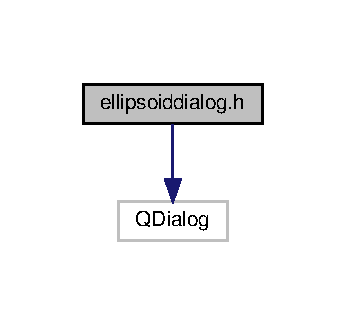
\includegraphics[width=166pt]{ellipsoiddialog_8h__incl}
\end{center}
\end{figure}
This graph shows which files directly or indirectly include this file\+:
\nopagebreak
\begin{figure}[H]
\begin{center}
\leavevmode
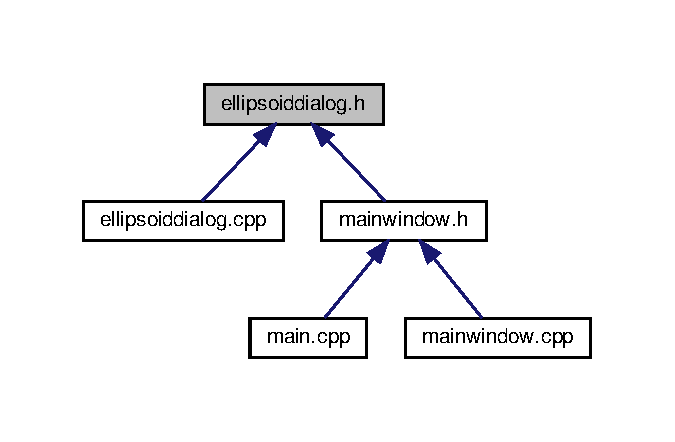
\includegraphics[width=324pt]{ellipsoiddialog_8h__dep__incl}
\end{center}
\end{figure}
\subsection*{Classes}
\begin{DoxyCompactItemize}
\item 
class \hyperlink{class_ellipsoid_dialog}{Ellipsoid\+Dialog}
\end{DoxyCompactItemize}
\subsection*{Namespaces}
\begin{DoxyCompactItemize}
\item 
 \hyperlink{namespace_ui}{Ui}
\end{DoxyCompactItemize}

\hypertarget{figurageometrica_8cpp}{}\section{figurageometrica.\+cpp File Reference}
\label{figurageometrica_8cpp}\index{figurageometrica.\+cpp@{figurageometrica.\+cpp}}
{\ttfamily \#include \char`\"{}figurageometrica.\+h\char`\"{}}\newline
Include dependency graph for figurageometrica.\+cpp\+:
\nopagebreak
\begin{figure}[H]
\begin{center}
\leavevmode
\includegraphics[width=187pt]{figurageometrica_8cpp__incl}
\end{center}
\end{figure}

\hypertarget{figurageometrica_8h}{}\section{figurageometrica.\+h File Reference}
\label{figurageometrica_8h}\index{figurageometrica.\+h@{figurageometrica.\+h}}
{\ttfamily \#include \char`\"{}sculptor.\+h\char`\"{}}\newline
Include dependency graph for figurageometrica.\+h\+:
\nopagebreak
\begin{figure}[H]
\begin{center}
\leavevmode
\includegraphics[width=177pt]{figurageometrica_8h__incl}
\end{center}
\end{figure}
This graph shows which files directly or indirectly include this file\+:
\nopagebreak
\begin{figure}[H]
\begin{center}
\leavevmode
\includegraphics[width=350pt]{figurageometrica_8h__dep__incl}
\end{center}
\end{figure}
\subsection*{Classes}
\begin{DoxyCompactItemize}
\item 
class \hyperlink{class_figura_geometrica}{Figura\+Geometrica}
\begin{DoxyCompactList}\small\item\em A classe \hyperlink{class_figura_geometrica}{Figura\+Geometrica} serce como classe abstrata para criação de outras figuras. \end{DoxyCompactList}\end{DoxyCompactItemize}

\hypertarget{main_8cpp}{}\section{main.\+cpp File Reference}
\label{main_8cpp}\index{main.\+cpp@{main.\+cpp}}
{\ttfamily \#include \char`\"{}mainwindow.\+h\char`\"{}}\newline
{\ttfamily \#include $<$Q\+Application$>$}\newline
Include dependency graph for main.\+cpp\+:
\nopagebreak
\begin{figure}[H]
\begin{center}
\leavevmode
\includegraphics[width=350pt]{main_8cpp__incl}
\end{center}
\end{figure}
\subsection*{Functions}
\begin{DoxyCompactItemize}
\item 
int \hyperlink{main_8cpp_a0ddf1224851353fc92bfbff6f499fa97}{main} (int argc, char $\ast$argv\mbox{[}$\,$\mbox{]})
\end{DoxyCompactItemize}


\subsection{Function Documentation}
\mbox{\Hypertarget{main_8cpp_a0ddf1224851353fc92bfbff6f499fa97}\label{main_8cpp_a0ddf1224851353fc92bfbff6f499fa97}} 
\index{main.\+cpp@{main.\+cpp}!main@{main}}
\index{main@{main}!main.\+cpp@{main.\+cpp}}
\subsubsection{\texorpdfstring{main()}{main()}}
{\footnotesize\ttfamily int main (\begin{DoxyParamCaption}\item[{int}]{argc,  }\item[{char $\ast$}]{argv\mbox{[}$\,$\mbox{]} }\end{DoxyParamCaption})}


\hypertarget{mainwindow_8cpp}{}\section{mainwindow.\+cpp File Reference}
\label{mainwindow_8cpp}\index{mainwindow.\+cpp@{mainwindow.\+cpp}}
{\ttfamily \#include \char`\"{}mainwindow.\+h\char`\"{}}\newline
{\ttfamily \#include \char`\"{}ui\+\_\+mainwindow.\+h\char`\"{}}\newline
Include dependency graph for mainwindow.\+cpp\+:
\nopagebreak
\begin{figure}[H]
\begin{center}
\leavevmode
\includegraphics[width=350pt]{mainwindow_8cpp__incl}
\end{center}
\end{figure}

\hypertarget{mainwindow_8h}{}\section{mainwindow.\+h File Reference}
\label{mainwindow_8h}\index{mainwindow.\+h@{mainwindow.\+h}}
{\ttfamily \#include \char`\"{}Q\+Debug\char`\"{}}\newline
{\ttfamily \#include \char`\"{}Q\+Message\+Box\char`\"{}}\newline
{\ttfamily \#include $<$Q\+Main\+Window$>$}\newline
{\ttfamily \#include \char`\"{}dimdialog.\+h\char`\"{}}\newline
{\ttfamily \#include \char`\"{}Q\+Color\char`\"{}}\newline
{\ttfamily \#include \char`\"{}boxdialog.\+h\char`\"{}}\newline
{\ttfamily \#include \char`\"{}spheredialog.\+h\char`\"{}}\newline
{\ttfamily \#include \char`\"{}Q\+Color\+Dialog\char`\"{}}\newline
{\ttfamily \#include \char`\"{}Q\+File\+Dialog\char`\"{}}\newline
{\ttfamily \#include \char`\"{}cstring\char`\"{}}\newline
{\ttfamily \#include \char`\"{}Q\+String\char`\"{}}\newline
{\ttfamily \#include \char`\"{}ellipsoiddialog.\+h\char`\"{}}\newline
Include dependency graph for mainwindow.\+h\+:
\nopagebreak
\begin{figure}[H]
\begin{center}
\leavevmode
\includegraphics[width=350pt]{mainwindow_8h__incl}
\end{center}
\end{figure}
This graph shows which files directly or indirectly include this file\+:
\nopagebreak
\begin{figure}[H]
\begin{center}
\leavevmode
\includegraphics[width=244pt]{mainwindow_8h__dep__incl}
\end{center}
\end{figure}
\subsection*{Classes}
\begin{DoxyCompactItemize}
\item 
class \hyperlink{class_main_window}{Main\+Window}
\end{DoxyCompactItemize}
\subsection*{Namespaces}
\begin{DoxyCompactItemize}
\item 
 \hyperlink{namespace_ui}{Ui}
\end{DoxyCompactItemize}

\hypertarget{plotter_8cpp}{}\section{plotter.\+cpp File Reference}
\label{plotter_8cpp}\index{plotter.\+cpp@{plotter.\+cpp}}
{\ttfamily \#include \char`\"{}plotter.\+h\char`\"{}}\newline
{\ttfamily \#include $<$Q\+Painter$>$}\newline
{\ttfamily \#include $<$Q\+Pen$>$}\newline
{\ttfamily \#include $<$Q\+Brush$>$}\newline
{\ttfamily \#include $<$Q\+Event$>$}\newline
{\ttfamily \#include $<$Q\+Debug$>$}\newline
{\ttfamily \#include \char`\"{}putvoxel.\+h\char`\"{}}\newline
{\ttfamily \#include \char`\"{}cutvoxel.\+h\char`\"{}}\newline
{\ttfamily \#include \char`\"{}putbox.\+h\char`\"{}}\newline
{\ttfamily \#include \char`\"{}cutbox.\+h\char`\"{}}\newline
{\ttfamily \#include \char`\"{}putsphere.\+h\char`\"{}}\newline
{\ttfamily \#include \char`\"{}cutsphere.\+h\char`\"{}}\newline
{\ttfamily \#include \char`\"{}putellipsoid.\+h\char`\"{}}\newline
{\ttfamily \#include \char`\"{}cutellipsoid.\+h\char`\"{}}\newline
Include dependency graph for plotter.\+cpp\+:
\nopagebreak
\begin{figure}[H]
\begin{center}
\leavevmode
\includegraphics[width=350pt]{plotter_8cpp__incl}
\end{center}
\end{figure}

\hypertarget{plotter_8h}{}\section{plotter.\+h File Reference}
\label{plotter_8h}\index{plotter.\+h@{plotter.\+h}}
{\ttfamily \#include $<$Q\+Widget$>$}\newline
{\ttfamily \#include $<$Q\+Action$>$}\newline
{\ttfamily \#include $<$sculptor.\+h$>$}\newline
{\ttfamily \#include $<$Q\+Mouse\+Event$>$}\newline
Include dependency graph for plotter.\+h\+:
\nopagebreak
\begin{figure}[H]
\begin{center}
\leavevmode
\includegraphics[width=350pt]{plotter_8h__incl}
\end{center}
\end{figure}
This graph shows which files directly or indirectly include this file\+:
\nopagebreak
\begin{figure}[H]
\begin{center}
\leavevmode
\includegraphics[width=304pt]{plotter_8h__dep__incl}
\end{center}
\end{figure}
\subsection*{Classes}
\begin{DoxyCompactItemize}
\item 
class \hyperlink{class_plotter}{Plotter}
\end{DoxyCompactItemize}

\hypertarget{putbox_8cpp}{}\section{putbox.\+cpp File Reference}
\label{putbox_8cpp}\index{putbox.\+cpp@{putbox.\+cpp}}
{\ttfamily \#include \char`\"{}putbox.\+h\char`\"{}}\newline
Include dependency graph for putbox.\+cpp\+:
\nopagebreak
\begin{figure}[H]
\begin{center}
\leavevmode
\includegraphics[width=177pt]{putbox_8cpp__incl}
\end{center}
\end{figure}

\hypertarget{putbox_8h}{}\section{putbox.\+h File Reference}
\label{putbox_8h}\index{putbox.\+h@{putbox.\+h}}
{\ttfamily \#include \char`\"{}figurageometrica.\+h\char`\"{}}\newline
Include dependency graph for putbox.\+h\+:
\nopagebreak
\begin{figure}[H]
\begin{center}
\leavevmode
\includegraphics[width=177pt]{putbox_8h__incl}
\end{center}
\end{figure}
This graph shows which files directly or indirectly include this file\+:
\nopagebreak
\begin{figure}[H]
\begin{center}
\leavevmode
\includegraphics[width=226pt]{putbox_8h__dep__incl}
\end{center}
\end{figure}
\subsection*{Classes}
\begin{DoxyCompactItemize}
\item 
class \hyperlink{class_put_box}{Put\+Box}
\begin{DoxyCompactList}\small\item\em A classe \hyperlink{class_put_box}{Put\+Box} implementa uma caixa no espaço. \end{DoxyCompactList}\end{DoxyCompactItemize}

\hypertarget{putellipsoid_8cpp}{}\section{putellipsoid.\+cpp File Reference}
\label{putellipsoid_8cpp}\index{putellipsoid.\+cpp@{putellipsoid.\+cpp}}
{\ttfamily \#include \char`\"{}putellipsoid.\+h\char`\"{}}\newline
Include dependency graph for putellipsoid.\+cpp\+:
\nopagebreak
\begin{figure}[H]
\begin{center}
\leavevmode
\includegraphics[width=177pt]{putellipsoid_8cpp__incl}
\end{center}
\end{figure}

\hypertarget{putellipsoid_8h}{}\section{putellipsoid.\+h File Reference}
\label{putellipsoid_8h}\index{putellipsoid.\+h@{putellipsoid.\+h}}
{\ttfamily \#include \char`\"{}figurageometrica.\+h\char`\"{}}\newline
Include dependency graph for putellipsoid.\+h\+:
\nopagebreak
\begin{figure}[H]
\begin{center}
\leavevmode
\includegraphics[width=177pt]{putellipsoid_8h__incl}
\end{center}
\end{figure}
This graph shows which files directly or indirectly include this file\+:
\nopagebreak
\begin{figure}[H]
\begin{center}
\leavevmode
\includegraphics[width=244pt]{putellipsoid_8h__dep__incl}
\end{center}
\end{figure}
\subsection*{Classes}
\begin{DoxyCompactItemize}
\item 
class \hyperlink{class_put_ellipsoid}{Put\+Ellipsoid}
\begin{DoxyCompactList}\small\item\em A classe \hyperlink{class_put_ellipsoid}{Put\+Ellipsoid} implementa um elipsoide no espaço. \end{DoxyCompactList}\end{DoxyCompactItemize}

\hypertarget{putsphere_8cpp}{}\section{putsphere.\+cpp File Reference}
\label{putsphere_8cpp}\index{putsphere.\+cpp@{putsphere.\+cpp}}
{\ttfamily \#include \char`\"{}putsphere.\+h\char`\"{}}\newline
Include dependency graph for putsphere.\+cpp\+:
\nopagebreak
\begin{figure}[H]
\begin{center}
\leavevmode
\includegraphics[width=177pt]{putsphere_8cpp__incl}
\end{center}
\end{figure}

\hypertarget{putsphere_8h}{}\section{putsphere.\+h File Reference}
\label{putsphere_8h}\index{putsphere.\+h@{putsphere.\+h}}
{\ttfamily \#include \char`\"{}figurageometrica.\+h\char`\"{}}\newline
Include dependency graph for putsphere.\+h\+:
\nopagebreak
\begin{figure}[H]
\begin{center}
\leavevmode
\includegraphics[width=177pt]{putsphere_8h__incl}
\end{center}
\end{figure}
This graph shows which files directly or indirectly include this file\+:
\nopagebreak
\begin{figure}[H]
\begin{center}
\leavevmode
\includegraphics[width=238pt]{putsphere_8h__dep__incl}
\end{center}
\end{figure}
\subsection*{Classes}
\begin{DoxyCompactItemize}
\item 
class \hyperlink{class_put_sphere}{Put\+Sphere}
\begin{DoxyCompactList}\small\item\em A classe \hyperlink{class_put_sphere}{Put\+Sphere} implementa uma esfera no espaço. \end{DoxyCompactList}\end{DoxyCompactItemize}

\hypertarget{putvoxel_8cpp}{}\section{putvoxel.\+cpp File Reference}
\label{putvoxel_8cpp}\index{putvoxel.\+cpp@{putvoxel.\+cpp}}
{\ttfamily \#include \char`\"{}putvoxel.\+h\char`\"{}}\newline
Include dependency graph for putvoxel.\+cpp\+:
\nopagebreak
\begin{figure}[H]
\begin{center}
\leavevmode
\includegraphics[width=177pt]{putvoxel_8cpp__incl}
\end{center}
\end{figure}

\hypertarget{putvoxel_8h}{}\section{putvoxel.\+h File Reference}
\label{putvoxel_8h}\index{putvoxel.\+h@{putvoxel.\+h}}
{\ttfamily \#include \char`\"{}figurageometrica.\+h\char`\"{}}\newline
Include dependency graph for putvoxel.\+h\+:
\nopagebreak
\begin{figure}[H]
\begin{center}
\leavevmode
\includegraphics[width=177pt]{putvoxel_8h__incl}
\end{center}
\end{figure}
This graph shows which files directly or indirectly include this file\+:
\nopagebreak
\begin{figure}[H]
\begin{center}
\leavevmode
\includegraphics[width=232pt]{putvoxel_8h__dep__incl}
\end{center}
\end{figure}
\subsection*{Classes}
\begin{DoxyCompactItemize}
\item 
class \hyperlink{class_put_voxel}{Put\+Voxel}
\begin{DoxyCompactList}\small\item\em A classe \hyperlink{class_put_voxel}{Put\+Voxel} implementa um voxel no espaço. \end{DoxyCompactList}\end{DoxyCompactItemize}

\hypertarget{_sculptor_8cpp}{}\section{Sculptor.\+cpp File Reference}
\label{_sculptor_8cpp}\index{Sculptor.\+cpp@{Sculptor.\+cpp}}
{\ttfamily \#include \char`\"{}sculptor.\+h\char`\"{}}\newline
{\ttfamily \#include $<$fstream$>$}\newline
{\ttfamily \#include $<$cmath$>$}\newline
Include dependency graph for Sculptor.\+cpp\+:
\nopagebreak
\begin{figure}[H]
\begin{center}
\leavevmode
\includegraphics[width=270pt]{_sculptor_8cpp__incl}
\end{center}
\end{figure}

\hypertarget{sculptor_8h}{}\section{sculptor.\+h File Reference}
\label{sculptor_8h}\index{sculptor.\+h@{sculptor.\+h}}
This graph shows which files directly or indirectly include this file\+:
\nopagebreak
\begin{figure}[H]
\begin{center}
\leavevmode
\includegraphics[width=350pt]{sculptor_8h__dep__incl}
\end{center}
\end{figure}
\subsection*{Classes}
\begin{DoxyCompactItemize}
\item 
struct \hyperlink{struct_voxel}{Voxel}
\begin{DoxyCompactList}\small\item\em O \hyperlink{struct_voxel}{Voxel} consiste em um cubo localizado no espaço tridimensional que possui cor, transparência e pode ou não estar ativado. \end{DoxyCompactList}\item 
class \hyperlink{class_sculptor}{Sculptor}
\begin{DoxyCompactList}\small\item\em A classe \hyperlink{class_sculptor}{Sculptor} define o espaço em que os voxels estarão alocados(como se fosse uma \char`\"{}prancheta\char`\"{} de desenho) \end{DoxyCompactList}\end{DoxyCompactItemize}

\hypertarget{spheredialog_8cpp}{}\section{spheredialog.\+cpp File Reference}
\label{spheredialog_8cpp}\index{spheredialog.\+cpp@{spheredialog.\+cpp}}
{\ttfamily \#include \char`\"{}spheredialog.\+h\char`\"{}}\newline
{\ttfamily \#include \char`\"{}ui\+\_\+spheredialog.\+h\char`\"{}}\newline
Include dependency graph for spheredialog.\+cpp\+:
\nopagebreak
\begin{figure}[H]
\begin{center}
\leavevmode
\includegraphics[width=270pt]{spheredialog_8cpp__incl}
\end{center}
\end{figure}

\hypertarget{spheredialog_8h}{}\section{spheredialog.\+h File Reference}
\label{spheredialog_8h}\index{spheredialog.\+h@{spheredialog.\+h}}
{\ttfamily \#include $<$Q\+Dialog$>$}\newline
Include dependency graph for spheredialog.\+h\+:
\nopagebreak
\begin{figure}[H]
\begin{center}
\leavevmode
\includegraphics[width=160pt]{spheredialog_8h__incl}
\end{center}
\end{figure}
This graph shows which files directly or indirectly include this file\+:
\nopagebreak
\begin{figure}[H]
\begin{center}
\leavevmode
\includegraphics[width=301pt]{spheredialog_8h__dep__incl}
\end{center}
\end{figure}
\subsection*{Classes}
\begin{DoxyCompactItemize}
\item 
class \hyperlink{class_sphere_dialog}{Sphere\+Dialog}
\end{DoxyCompactItemize}
\subsection*{Namespaces}
\begin{DoxyCompactItemize}
\item 
 \hyperlink{namespace_ui}{Ui}
\end{DoxyCompactItemize}

%--- End generated contents ---

% Index
\backmatter
\newpage
\phantomsection
\clearemptydoublepage
\addcontentsline{toc}{chapter}{Index}
\printindex

\end{document}
